%%%%%%%%%%%%%%%%%%%%%%%%%%%%%%%%%%%%%%%%%
% Bachelor/Master Thesis 
% LaTeX Template
% Version 2.5 (27/8/17)
%
% This template was downloaded from:
% http://www.LaTeXTemplates.com
%
% Version 2.x major modifications by:
% Vel (vel@latextemplates.com)
%
% This template is based on a template by:
% Steve Gunn (http://users.ecs.soton.ac.uk/srg/softwaretools/document/templates/) 
% Sunil Patel (http://www.sunilpatel.co.uk/thesis-template/)
% 
% Modified by Rostysav Hryniv (2019) and Oleg Farenyuk (2024) 
% 
% Template license:
% CC BY-NC-SA 3.0 (http://creativecommons.org/licenses/by-nc-sa/3.0/)
%
%%%%%%%%%%%%%%%%%%%%%%%%%%%%%%%%%%%%%%%%%

%----------------------------------------------------------------------------------------
%	PACKAGES AND OTHER DOCUMENT CONFIGURATIONS
%----------------------------------------------------------------------------------------

\documentclass[
    11pt, % The default document font size, options: 10pt, 11pt, 12pt
    oneside, % Two side (alternating margins) for binding by default, uncomment to switch to one side
    ukrainian,
    english, % ngerman for German
    singlespacing, % Single line spacing, alternatives: onehalfspacing or doublespacing
%draft, % Uncomment to enable draft mode (no pictures, no links, overfull hboxes indicated)
%nolistspacing, % If the document is onehalfspacing or doublespacing, uncomment this to set spacing in lists to single
%liststotoc, % Uncomment to add the list of figures/tables/etc to the table of contents
%toctotoc, % Uncomment to add the main table of contents to the table of contents
%parskip, % Uncomment to add space between paragraphs
%nohyperref, % Uncomment to not load the hyperref package
    headsepline, % Uncomment to get a line under the header
%chapterinoneline, % Uncomment to place the chapter title next to the number on one line
%consistentlayout, % Uncomment to change the layout of the declaration, abstract and acknowledgements pages to match the default layout
]{BachelorMasterThesis} % The class file specifying the document structure

\usepackage[utf8]{inputenc} % Required for inputting international characters
\usepackage[T1, T2A]{fontenc} % Output font encoding for international characters

\usepackage[ukrainian, english]{babel}

% \usepackage{mathpazo} % Use the Palatino font by default 
% O.F. Breaks Cyrillic, including Ukrainian, breaks bold, italic, etc. Commented out. The alternative is to use Lualatex.

\usepackage[backend=bibtex,natbib=true,maxbibnames=9,maxcitenames=2]{biblatex} % Use the bibtex backend with the authoryear citation style (which resembles APA)

\addbibresource{bibliography.bib} % The filename of the bibliography

\usepackage[autostyle=true]{csquotes} % Required to generate language-dependent quotes in the bibliography

\usepackage{amsmath}
\usepackage{amssymb}
\usepackage{enumitem}
\usepackage{todonotes}
\usepackage{subcaption}
\usepackage{bookmark}
\usepackage{mathtools}

\usepackage{datetime}

%----------------------------------------------------------------------------------------
%	MARGIN SETTINGS
%----------------------------------------------------------------------------------------

\geometry{
    paper=a4paper, % Change to letterpaper for US letter
    inner=2.5cm, % Inner margin
    outer=3.8cm, % Outer margin
    bindingoffset=.5cm, % Binding offset
    top=1.5cm, % Top margin
    bottom=1.5cm, % Bottom margin
%showframe, % Uncomment to show how the type block is set on the page
}

%----------------------------------------------------------------------------------------
%	THESIS INFORMATION
%----------------------------------------------------------------------------------------

\thesistitle{Practical Aspects of Recognising~Outer~\texorpdfstring{\(k\)}{k}-Planar~Graphs} % Your thesis title, this is used in the title and abstract, print it elsewhere with \ttitle
\supervisor{Prof. Dr. Alexander \textsc{Wolff}} % Your supervisor's name, this is used in the title page, print it elsewhere with \supname
\examiner{} % Your examiner's name, this is not currently used anywhere in the template, print it elsewhere with \examname
\degree{Bachelor of Science} % Your degree name, this is used in the title page and abstract, print it elsewhere with \degreename
\author{Ivan \textsc{Shevchenko}} % Your name, this is used in the title page and abstract, print it elsewhere with \authorname
\addresses{} % Your address, this is not currently used anywhere in the template, print it elsewhere with \addressname

\subject{Data Science} % Your subject area, this is not currently used anywhere in the template, print it elsewhere with \subjectname
\keywords{} % Keywords for your thesis, this is not currently used anywhere in the template, print it elsewhere with \keywordnames
\university{\href{http://www.ucu.edu.ua}{Ukrainian Catholic University}} % Your university's name and URL, this is used in the title page and abstract, print it elsewhere with \univname
\department{\href{http://apps.ucu.edu.ua}{Faculty of Applied Sciences}} % Your department's name and URL, this is used in the title page and abstract, print it elsewhere with \deptname
\group{\href{http://apps.ucu.edu.ua}{Department of Computer Sciences and Information Technologies}} % Your research group's name and URL, this is used in the title page, print it elsewhere with \groupname
\faculty{\href{http://apps.ucu.edu.ua}{}} % Your faculty's name and URL, this is used in the title page and abstract, print it elsewhere with \facname

\AtBeginDocument{
    \hypersetup{pdftitle=\ttitle} % Set the PDF's title to your title
    \hypersetup{pdfauthor=\authorname} % Set the PDF's author to your name
    \hypersetup{pdfkeywords=\keywordnames} % Set the PDF's keywords to your keywords
}

\begin{document}

    \frontmatter % Use roman page numbering style (i, ii, iii, iv...) for the pre-content pages

    \pagestyle{plain} % Default to the plain heading style until the thesis style is called for the body content

%----------------------------------------------------------------------------------------
%	TITLE PAGE
%----------------------------------------------------------------------------------------

    \begin{titlepage}
        \begin{center}

            \vspace*{.06\textheight}
            {\scshape\LARGE \univname\par}\vspace{1.5cm} % University name
            \textsc{\Large Bachelor Thesis}\\[0.5cm] % Thesis type

            \HRule \\[0.4cm] % Horizontal line
            {\huge \bfseries \ttitle\par}\vspace{0.4cm} % Thesis title
            \HRule \\[1.5cm] % Horizontal line

            \begin{minipage}[t]{0.4\textwidth}
                \begin{flushleft}
                    \large
                    \emph{Author:}\\
                    \href{https://www.linkedin.com/in/ishevche/}{\authorname} % Author name - remove the \href bracket to remove the link
                \end{flushleft}
            \end{minipage}
            \begin{minipage}[t]{0.4\textwidth}
                \begin{flushright}
                    \large
                    \emph{Supervisor:} \\
                    \href{https://www.informatik.uni-wuerzburg.de/algo/team/wolff-alexander/}{\supname} % Supervisor name - remove the \href bracket to remove the link
                \end{flushright}
            \end{minipage}\\[3cm]

            \vfill

            \large \textit{A thesis submitted in fulfillment of the requirements\\ for the degree of \degreename}\\[0.3cm] % University requirement text
            \textit{in the}\\[0.4cm]
            \groupname\\\deptname\\[2cm] % Research group name and department name

            \vfill
            
\includegraphics[height=2.5cm]{UCU_APPS_logo} % University/department logo - uncomment to place it
% Logo taken from the official brandbook: https://ucu.edu.ua/brandbook/brand-book-sources/
% UCU_APPS_logo.pdf 

            \vfill
            {\large Lviv 2025}\\{\today\quad\currenttime}\\[4cm] % Date

            \vfill
        \end{center}
    \end{titlepage}

%----------------------------------------------------------------------------------------
%	DECLARATION PAGE
%----------------------------------------------------------------------------------------
%
%    \begin{declaration}
%        \addchaptertocentry{\authorshipname} % Add the declaration to the table of contents
%        \noindent I, \authorname, declare that this thesis titled, \enquote{\ttitle} and the work presented in it are my own. I confirm that:
%
%        \begin{itemize}
%            \item This work was done wholly or mainly while in candidature for a research degree at this University.
%            \item Where any part of this thesis has previously been submitted for a degree or any other qualification at this University or any other institution, this has been clearly stated.
%            \item Where I have consulted the published work of others, this is always clearly attributed.
%            \item Where I have quoted from the work of others, the source is always given. With the exception of such quotations, this thesis is entirely my own work.
%            \item I have acknowledged all main sources of help.
%            \item Where the thesis is based on work done by myself jointly with others, I have made clear exactly what was done by others and what I have contributed myself.\\
%        \end{itemize}
%
%        \noindent Signed:\\
%        \rule[0.5em]{25em}{0.5pt} % This prints a line for the signature
%
%        \noindent Date:\\
%        \rule[0.5em]{25em}{0.5pt} % This prints a line to write the date
%    \end{declaration}
%
%    \cleardoublepage

%----------------------------------------------------------------------------------------
%	QUOTATION PAGE 
%----------------------------------------------------------------------------------------

%\vspace*{0.2\textheight}

%\noindent\enquote{\itshape Thanks to my solid academic training, today I can write hundreds of words on virtually any topic without possessing a shred of information, which is how I got a good job in journalism.}\bigbreak

%\hfill Dave Barry

%----------------------------------------------------------------------------------------
%	ABSTRACT PAGE
%----------------------------------------------------------------------------------------

    \begin{abstract}
        \addchaptertocentry{\abstractname} % Add the abstract to the table of contents
        The Thesis Abstract is written here (and usually kept to just this page). The page is kept centered vertically so can expand into the blank space above the title too\ldots
    \end{abstract}

%----------------------------------------------------------------------------------------
%	ACKNOWLEDGEMENTS
%----------------------------------------------------------------------------------------

    \begin{acknowledgements}
        \addchaptertocentry{\acknowledgementname} % Add the acknowledgements to the table of contents
        The acknowledgments and the people to thank go here, don't forget to include your project advisor\ldots
    \end{acknowledgements}

%----------------------------------------------------------------------------------------
%	LIST OF CONTENTS/FIGURES/TABLES PAGES
%----------------------------------------------------------------------------------------

    \tableofcontents % Prints the main table of contents

%\listoffigures % Prints the list of figures

%\listoftables % Prints the list of tables

%----------------------------------------------------------------------------------------
%	ABBREVIATIONS
%----------------------------------------------------------------------------------------

%\begin{abbreviations}{ll} % Include a list of abbreviations (a table of two columns)

%\textbf{LAH} & \textbf{L}ist \textbf{A}bbreviations \textbf{H}ere\\
%\textbf{WSF} & \textbf{W}hat (it) \textbf{S}tands \textbf{F}or\\

%\end{abbreviations}

%----------------------------------------------------------------------------------------
%	PHYSICAL CONSTANTS/OTHER DEFINITIONS
%----------------------------------------------------------------------------------------

%\begin{constants}{lr@{${}={}$}l} % The list of physical constants is a three column table

% The \SI{}{} command is provided by the siunitx package, see its documentation for instructions on how to use it

%Speed of Light & $c_{0}$ & \SI{2.99792458e8}{\meter\per\second} (exact)\\
%Constant Name & $Symbol$ & $Constant Value$ with units\\

%\end{constants}

%----------------------------------------------------------------------------------------
%	SYMBOLS
%----------------------------------------------------------------------------------------

%\begin{symbols}{lll} % Include a list of Symbols (a three column table)

%$a$ & distance & \si{\meter} \\
%$P$ & power & \si{\watt} (\si{\joule\per\second}) \\
%Symbol & Name & Unit \\

%\addlinespace % Gap to separate the Roman symbols from the Greek

%$\omega$ & angular frequency & \si{\radian} \\

%\end{symbols}

%----------------------------------------------------------------------------------------
%	DEDICATION
%----------------------------------------------------------------------------------------

%\dedicatory{For/Dedicated to/To my\ldots}

%----------------------------------------------------------------------------------------
%	THESIS CONTENT - CHAPTERS
%----------------------------------------------------------------------------------------

    \mainmatter % Begin numeric (1,2,3...) page numbering

    \pagestyle{thesis} % Return the page headers back to the "thesis" style

% Include the chapters of the thesis as separate files from the Chapters folder
% Uncomment the lines as you write the chapters
% Remember -- some filesystems are case sensitive.

    \chapter{Introduction}\label{ch:introduction}

Nowadays, graphs are widely used across different domains and occupation. They prove to be an efficient tool for visualising relational systems. However, as the size of the graphs grows, so does their complexity, which makes understanding their internal structure increasingly difficult.

This problem was acknowledged by the community as early as in the~1980s. One of the key points, discussed by the researchers in the field was the importance of reducing the edge crossings for improving visual clarity~\cite{early-few-crossing}. The suspicion that a drawing with fewer edge crossings was easier to comprehend was later confirmed by several experimental studies~\cite{graph-aesthetic-survey}. These studies showed that minimising the crossings in graph representations significantly improves the ability of humans to interpret the structure, particularly when dealing with complex or large graphs.

This led to exploration of the ideal form for crossing minimising drawings~--~planar ones. However, requiring the drawing to be completely crossing free imposes severe limitations on an underlying graph. While providing a clean structure, these restrictions are often too constraining for many real-world graphs, especially large ones. As a consequence, many processes cannot be represented in a planar manner, so no insights acquired by the decades-long studies are applicable to them.

As a result, research community expresses the growing interest in exploring graphs which drawings are beyond planar; see the survey by \citeauthor{beyond-planarity-survey}~\cite{beyond-planarity-survey}. This led to exploration of alternative approaches for eliminating edge crossings, such as drawings which include only parts of the edges~\cite{break-the-edge,break-the-edge2}, or merge several edges to form a single track~\cite{confluent-drawings}. However, the most popular approach is to consider \emph{almost} planar graphs~--~graphs which admit a drawing with a limited number of crossings. Such graphs offer a balance between visual recognisability and structural flexibility, while still retaining some of the beneficial structural properties of planar graphs.

The most natural way to impose a limit on the amount of crossing is to bound the number of crossings for each edge by some value \(k\). This class of graphs is among those that have attracted the most interest from the research community lately~\cite{contest}.\todo{How do I explain why We have done this step?} In this work, however, we went a step further, additionally limiting the vertices to lie on a single (outer) face of the drawing. Such drawings that comply with both limitations are called outer \(k\)-planar, and so do the graphs, which admit such drawings.


\section{Our contribution}

However, despite all recent advances in this area, all studies are conducted in a theoretical context and were not implemented or tested empirically. Thus, all discussed methods lack practical validation. In this thesis we want to address this gap by implementing the most recent recognition algorithm and introducing two alternative approaches based on Integer Linear Programming (ILP) and Satisfiability (SAT) problems. While it is NP-hard to solve the general integer linear programming problem or to find a satisfying truth assignment for general Boolean formulas, there are very advanced solvers that can help us find the exact solutions for small- to medium-sized instances within an acceptable amount of time. We also evaluate the performance and efficiency of these methods, demonstrating their practical applicability and their limitations.


\section{Structure of the thesis}

\begin{itemize}
    \item \Cref{ch:related-work} discusses the current state of the research by reviewing the key works in the context of planar and almost planar graph drawings. Here, we also discuss the complexity of the problem.
    \item \Cref{ch:proposed-solution} describes three algorithms for recognising outer \(k\)-planar graphs. Additionally, it presents the optimisations we used to improve the performance of the implemented methods.
    \item \Cref{ch:experiments-and-results} demonstrates the results of the implemented algorithms. It also describes the experiments we conducted to evaluate the performance and discusses the obtained results.
    \item \Cref{ch:conclusions} summarises the key accomplishments and overviews the results. It also discusses the limitations and outlines potential improvements that can be made to overcome them.
\end{itemize}
    \chapter{Related Work}\label{ch:related-work}

As we discussed in~\Cref{ch:introduction}, to get the easily interpretable graph, its drawing should minimise the number of crossings. The first algorithms, designed to do so programmatically, were designed to recognise planar graphs, and construct a drawing for those who admit such. The first linear-time algorithm for doing so was introduced as early as~\citeyear{linear-p} by \citeauthor{linear-p}~\cite{linear-p}. In this chapter we discuss studies that address the recognition problem for almost planar graphs.

\section{Difficulty of dealing with beyond-planar graphs}

Most relaxations of strict planarity dramatically increase the complexity of recognising such graphs. So, the general problem of minimising edge crossings in a graph drawing was known to be computationally intractable already in~\citeyear{cr_NPC} when \citeauthor{cr_NPC}~\cite{cr_NPC} demonstrated that the \textsc{Crossing Number} problem, where the task is to check whether a given graph can be drawn with at most \(k\) crossings, is NP-hard. Their proof relies on a reduction from the \textsc{Optimal Linear Arrangement} problem, which is known to be NP-hard.

Minimising the number of local crossings is also hard. \citeauthor{1p-NPH}~\cite{1p-NPH} showed that testing \(1\)-planarity, that is, recognising whether a graph can be drawn with at most one crossing per edge, is NP-hard. Later, \citeauthor{one-edge-NPH}~\cite{one-edge-NPH} showed that testing~\(1\)-planarity is NP-hard even for near-planar graphs, that is, graphs that can be obtained from planar graphs by adding a single edge.

\begin{figure}[tbh]
    \centering
    \captionsetup{subrefformat=parens}
    \subfloat[\(1\)-planar drawing]{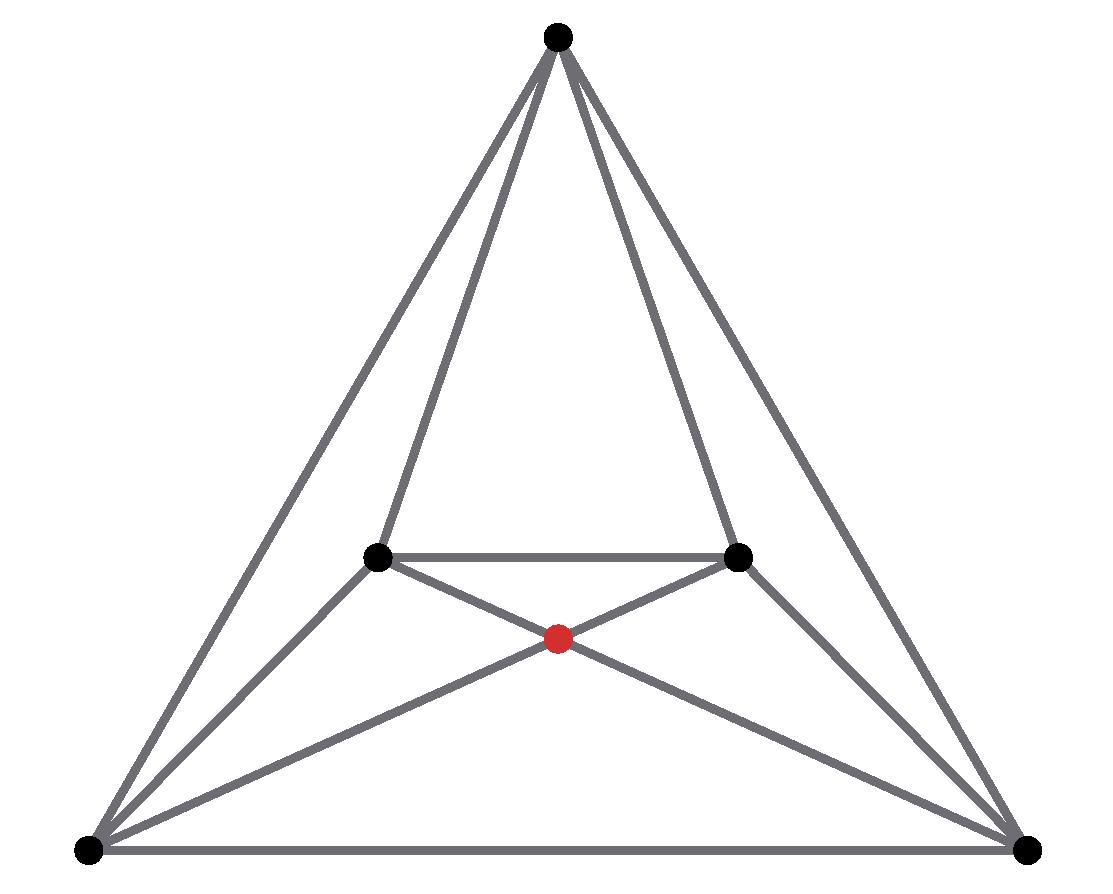
\includegraphics[width=0.3\textwidth]{k5_1planar}\label{fig:k5:1-planar}}
    \subfloat[Outer \(2\)-planar drawing]{
\includegraphics[width=0.3\textwidth]{k5_outer2planar}\label{fig:k5:o2p}}
    \caption{Drawing of \(K_5\) \subref{fig:k5:1-planar}~non-restricted and \subref{fig:k5:o2p}~restricted to a circular setting.}
    \label{fig:figure}
\end{figure}

Given the complexity of recognising \(k\)-planarity, researchers have considered exploring more restrictive settings, hoping that the imposed limitations could simplify the recognition. One of the considered restrictions is a circular setting that requires the vertices to be placed on a circle and the edges to be drawn as straight lines. This restriction gives rise to the \emph{circular local crossing number} of a graph, which we study in this thesis. The graphs whose circular crossing number is bounded by \(k\) are called \emph{outer \(k\)-planar} graphs. For example, \(K_5\), the complete graph with five vertices, is known to be the smallest non-planar graph. It can be drawn with a single crossing, hence it is \(1\)-planar (see~\Cref{fig:k5:1-planar}). When insisting on the circular setting, however, every second edge receives two crossings, hence \(K_5\) is outer \(2\)-planar (see~\Cref{fig:k5:o2p}).


\section{Efficient recognition of some outer \texorpdfstring{\(k\)}{k}-planar graphs}

Although the recognition problem for outer \(k\)-planar graphs is NP-hard if \(k\) is a part of the input, efficient algorithms have been developed for any constant value of \(k\).

For \(k = 0\), the recognition task simplifies to an outerplanarity test. Recognition can be accomplished by augmenting the graph with a new vertex connected to all original vertices and testing whether the resulting graph is planar. An alternative approach, described in~\cite{linear-op}, introduces the concept of~\(2\)-reducible graphs, which are totally disconnected or can be made totally disconnected by repeated deletion of edges adjacent to a vertex with a degree at most two. The proposed outerplanarity test is based on an algorithm for testing~\(2\)-reducibility.

In the case of \(k = 1\), two research groups independently presented linear-time algorithms~\cite{linear-o1p_, linear-o1p}. Both algorithms use the SPQR decomposition of a graph for the test. Notably, the latter solution extends the graph to a maximal outer~\(1\)-planar configuration if such a drawing exists, unlike the former, which employs a bottom-up strategy which does not require any transformations of the original graph.

Considering a special case of this problem, \citeauthor{linear-full-o2p}~\cite{linear-full-o2p} proposed a linear-time algorithm for recognising full outer~\(2\)-planar graphs. An outer \(k\)-planar drawing is \emph{full} if no crossings lie on the boundary of the outer face. Later, \citeauthor{linear-full-okp}~\cite{linear-full-okp} extended their result by introducing an algorithm for recognising full outer \(k\)-planar graphs for every \(k\). Their algorithm runs in \(O(f(k) \cdot n)\) time, where \(f\) is a computable function.

For the general version of the problem and values of \(k > 1\), no research was conducted until recently when a group of researchers proposed an algorithm for the general case, which we discuss in the~\Cref{sec:recognising-general-outer-(k)-planar-graphs}.


\section{Recognising general outer \texorpdfstring{\(k\)}{k}-planar graphs}\label{sec:recognising-general-outer-(k)-planar-graphs}

For a given outer \(k\)-planar drawing of a graph, \citeauthor{triangulations}~\cite{triangulations} proposed a method for constructing a triangulation with the property that each edge of the triangulation is crossed by at most \(k\) edges of the graph drawing. Since the edges of the triangulation do not necessarily belong to the original graph, they are termed \emph{links} to distinguish them from the original graph edges. The construction is done recursively.

Initially, the algorithm selects an edge on the outer face and labels it as the active link. At each recursive step, the active link partitions the graph into two regions: a left part already triangulated and a right part not yet explored. The objective of each step is to triangulate the right portion. To achieve this, a splitting vertex is chosen within the right region, dividing it into two smaller subregions. The splitting vertex is selected so that the two new links, connecting the split vertex with the endpoints of the active link, are each intersected by at most \(k\) edges, which allows including them into the triangulation. The algorithm then recurses, treating each of these newly formed links as the active one.

Later, \citeauthor{okp}~\cite{okp} extended this approach to address the recognition problem for outer \(k\)-planar graphs. In contrast to the triangulation task, where the drawing is provided, the recognition problem requires determining whether a given graph admits an outer \(k\)-planar drawing. Although the core idea remains analogous, the absence of a drawing requires the exploration of all possible configurations. Here, each recursive step verifies whether the unexplored right portion of the graph can be drawn as an outer \(k\)-planar graph that is compatible with the left part.

Moreover, instead of relying on recursion, the method utilises a dynamic programming approach. This framework combines solutions of smaller subproblems retrieved from a table to solve larger ones. To populate this table, the algorithm iterates over all possible configurations corresponding to different recursion steps. Several parameters characterise each such configuration. The first parameter is the active link~--~a pair of vertices that divides the graph into a left and a right region. The second parameter is a set of vertices in the right part, which is not uniquely determined as in the triangulation case. Additionally, the configuration depends on the order in which edges intersect the active link and the number of intersections on the right side for each one of them. These parameters are used to ensure that the drawing of the right part is compatible with the left part. For each configuration, the algorithm considers all possible ways to split the right region further. For each of them, the method checks whether these splits are compatible with each other and the left part of the drawing.

Using the restriction on the number of edges crossing each link, the authors demonstrated that for a fixed \(k\), the number of possible right subgraphs grows only polynomially with respect to the size of the graph. They proceeded by arguing that the overall time complexity of the algorithm is~\(2^{O(k \log k)}n^{3k + O(1)}\), showing that the algorithm is efficient for any fixed parameter \(k\). This indicates that this problem belongs to the XP class~--~a class of problems that admit such ``slicewise polynomial'' algorithms.


\section{Our contribution}

A common drawback of the methods described above is the lack of practical validation. Although these algorithms have been analysed and discussed in a theoretical context, they have not been implemented or tested empirically. We address this gap by implementing the most recent recognition algorithm and introducing two alternative approaches based on Integer Linear Programming (ILP) and Satisfiability (SAT) formulations. While it is NP-hard to solve the general integer linear programming problem or to find a satisfying truth assignment for general Boolean formulas, there are very advanced solvers for such formulations that allow us to find exact solutions for small- to medium-sized instances within an acceptable amount of time. We evaluate the performance and efficiency of these methods, demonstrating their practical applicability and their limitations.

%\chapter{Theoretical Background }
    \chapter{Proposed Solution}

This chapter will discuss the methods this work considers to recognise the outer \(k\)-planar graphs. Besides recognition, these methods provide the outer \(k\)-planar drawings of the given graphs if possible. We represent the drawing as a sequence of vertices in the circular order they appear on the boundary of the outer face. Considering only straight-line drawings, this order uniquely determines all the edge crossings and, thus, also the number of crossings per edge.


\section{Bicomponent decomposition}

For complex problems, decomposing into smaller, independent subproblems often leads to a significant performance boost. In our context of recognising outer \(k\)-planar graphs, an effective strategy to do so is to partition the graph into subgraphs in such a manner that allows us to process them independently by the recognition algorithm. As the smallest part of the graph that can be processed by any algorithm independently of the remainder is a biconnected component, we use block-cut decomposition for this purpose, which splits the graph into biconnected components, referred to as blocks. It is worth noting that each graph edge belongs to a single block. However, any two bicomponents may share a vertex, referred to as a cut vertex. Considering blocks and cut vertices as graph nodes, we can construct a so-called block-cut tree, wherein a block node is connected to a cut node if and only if the corresponding biconnected component contains a corresponding vertex.

The advantage of this decomposition is that any method for recognising outer \(k\)-planar graphs can be applied separately to each component, and results can be combined easily afterwards. Specifically, if some component does not admit an outer \(k\)-planar drawing, neither does the whole graph. Otherwise, if all components admit such a drawing, they can be merged by combining duplicates of each cut vertex. This merging process does not introduce any additional edge crossings since both components are located on the outer face of each other. Moreover, as no new faces are created during this process -- due to the acyclic structure of the block-cut tree -- every vertex remains on the outer face of the graph during this process. Consequently, the resulting drawing of an original graph is outer \(k\)-planar, and it exists if and only if each biconnected component of the graph admits such a drawing.

In this work, we implemented this decomposition using the method \textsf{biconnected\_compo\-nents}\footnote{\url{https://www.boost.org/doc/libs/1_87_0/libs/graph/doc/biconnected_components.html}} from the Boost Graph Library~\cite{boost}. This function assigns an index of the bicomponent to each edge to which it belongs. Additionally, it provides a list of cut vertices. Afterwards, we copy each block as an independent graph and create mappings to translate new \emph{local} vertices back to their original identifiers. Finally, we construct a supergraph representing the structure of a block-cut tree wherein each node references a copied block along with corresponding mapping or a cut vertex.

To construct a final graph drawing, we perform a depth-first search on the block-cut tree, recording the predecessor for each node upon discovery. Also, each time a block vertex is discovered, we use one of the methods described in other sections of this chapter to check whether the component admits an outer \(k\)-planar drawing and obtain it if so. Afterwards, we merge the new drawing with the already existing one by combining the corresponding cut vertex as described before. If the considered block is the first encountered one, its drawing is directly copied into a sequence that will form the final drawing. Otherwise, the block necessarily has a predecessor. Due to the structure of a tree, it is a cut node corresponding to a vertex that is shared with some other block that has already been considered and thus added to a final drawing. As a result, we can find a corresponding cut vertex in both global and local drawings. Since each drawing is represented as a cyclic sequence of vertices, we can rotate the local drawing so that the corresponding cut vertex appears as the first item in a sequence. Finally, we insert the local drawing starting from the second element into the global one immediately after the cut vertex.

\section{ILP Formulation (unchanged)}\label{sec:ILP-def}

The result of the integral linear program should be an arrangement of vertices on a line.
Given the arrangement of the vertices, we can definitively identify whether two edges cross each other.
Indeed, consider two edges, $uv$ and $st$.
Without loss of generality, we can assume that $u$ is located before $v$ in the arrangement, $s$ before $t$, and $u$ before $s$.
Under these assumptions, the edges $uv$ and $st$ cross if and only if $s$ is located before $v$ and $t$ after $v$.

\todo[inline]{Image depicting 8 intersecting pairs out of 24 possibble}

The arrangement is represented using the so-called ``ordering variables''.
For every pair of vertices $u$ and $v$, we create a binary variable $a_{u, v}$ that defines the order in which they appear in the arrangement.
Equality $a_{u, v} = 1$ indicates that $u$ is located before $v$ and vice versa, and $a_{u, v} = 0$ indicates that $v$ is located before $u$ or $u$ and $v$ is the same vertex.

For these variables, it is crucial to ensure transitivity.
That is, if $a_{u, v} = 1$ and $a_{v, w} = 1$ which means $u$ is located before $v$ and $v$ is located before $w$, then $u$ must be located before $w$, so the following should hold $a_{u, w} = 1$.
This can be ensured by the following constraint: $a_{u, w} \geqslant a_{u, v} + a_{v, w} - 1$.
This constraint will restrict the value of $a_{u, w}$ if and only if both $a_{u, v}$ and $a_{v, w}$ equal $1$.
Otherwise, the constraint will have no impact on the system at all.

Having the arrangement of the vertices, we can now deduce for each pair of edges $uv$ and $st$ whether they intersect or not.
Naturally, there are 24 different arrangements of the vertices, as demonstrated in figure~\ref{fig:edge_crossings}.
Among them, there are only eight in which the edges intersect.
Thus, the edge $uv$ crosses the edge $st$ if and only if one of the following holds:
\begin{itemize}[noitemsep]
    \item $a_{u,s} = 1$, $a_{s,v} = 1$, and $a_{v,t} = 1$
    \item $a_{u,t} = 1$, $a_{t,v} = 1$, and $a_{v,s} = 1$
    \item $a_{v,s} = 1$, $a_{s,u} = 1$, and $a_{u,t} = 1$
    \item $a_{v,t} = 1$, $a_{t,u} = 1$, and $a_{u,s} = 1$
    \item $a_{s,u} = 1$, $a_{u,t} = 1$, and $a_{t,v} = 1$
    \item $a_{t,u} = 1$, $a_{u,s} = 1$, and $a_{s,v} = 1$
    \item $a_{s,v} = 1$, $a_{v,t} = 1$, and $a_{t,u} = 1$
    \item $a_{t,v} = 1$, $a_{v,s} = 1$, and $a_{s,u} = 1$
\end{itemize}

To describe this in the linear program, we create a binary variable $c_{uv, st}$ for every pair of edges $uv$ and $st$.
Equality $c_{uv, st} = 0$ indicates that the edge $uv$ does not cross $st$.
To ensure the correctness of these values, we impose eight constraints on each variable, one for each case from above.
For example, considering the case $a_{u,s} = 1$, $a_{s,v} = 1$, and $a_{v,t} = 1$, we impose the following restriction: $c_{uv, st} \geqslant a_{u,s} + a_{s,v} + a_{v,t} - 2$, which ensures that $c_{uv, st}$ equals $1$ whenever the vertices are ordered as $usvt$.
Making this for each case restricts $c_{uv, st}$ to the value $1$ if the vertices are arranged in one of the eight ``intersecting'' configurations, ensuring that $c_{uv, st} = 0$ is possible only if $uv$ does not cross $st$.

The algorithm's objective is to minimize the maximal number of crossings per edge.
This value can be written as follows: $\max_{uv \in E(G)} \sum_{st \in E(G)} c_{uv, st}$.
Unfortunately, it cannot represent an objective function for a linear program as the $\max$ operation is not linear.
To solve this, we introduce a new integer variable $k$.
To ensure that it is equal to the objective value, we impose the following constraint on $k$: $k \geqslant \sum_{st \in E(G)} c_{uv, st}$ for each edge $uv \in E(G)$.

So, the integer linear program can be described as follows:
\begin{align*}
    \textbf{minimize}\quad&k\\
    \textbf{subject to}\quad&&k &\geqslant \sum_{st \in E(G)} c_{uv, st},&&\forall uv \in E(G)\\
    &&c_{uv, st} &\geqslant a_{u,s} + a_{s,v} + a_{v,t} - 2,&&\forall uv, st \in E(G)\\
    &&c_{uv, st} &\geqslant a_{u,t} + a_{t,v} + a_{v,s} - 2,&&\forall uv, st \in E(G)\\
    &&c_{uv, st} &\geqslant a_{v,s} + a_{s,u} + a_{u,t} - 2,&&\forall uv, st \in E(G)\\
    &&c_{uv, st} &\geqslant a_{v,t} + a_{t,u} + a_{u,s} - 2,&&\forall uv, st \in E(G)\\
    &&c_{uv, st} &\geqslant a_{s,u} + a_{u,t} + a_{t,v} - 2,&&\forall uv, st \in E(G)\\
    &&c_{uv, st} &\geqslant a_{t,u} + a_{u,s} + a_{s,v} - 2,&&\forall uv, st \in E(G)\\
    &&c_{uv, st} &\geqslant a_{s,v} + a_{v,t} + a_{t,u} - 2,&&\forall uv, st \in E(G)\\
    &&c_{uv, st} &\geqslant a_{t,v} + a_{v,s} + a_{s,u} - 2,&&\forall uv, st \in E(G)\\
    &&a_{u, w} &\geqslant a_{u, v} + a_{v, w} - 1,&&\forall u, v, w \in V(G)\\
    &&c_{uv, st} &\in \{0, 1\},&&\forall uv, st \in E(G)\\
    &&a_{u, v} &\in \{0, 1\},&&\forall u, v \in V(G)\\
\end{align*}

\section{SAT Formulation (unchanged)}\label{sec:SAT-def}

Another approach to solving this problem is to check for a specific $k$ whether the given graph is outer-$k$-planar.
This check can be encoded as a boolean satisfiability problem.
This problem asks whether it is possible to assign logic values $\textsc{True}$ or $\textsc{False}$ so that all disjunctive clauses are satisfied.
A disjunctive clause is a single literal or a disjunction of several.
Literal is either a variable or a negation of a variable, with the former being the positive and the latter the negative literal.


Similarly to the ILP algorithm described in~\ref{sec:ILP-def}, this algorithm uses the same ``ordering variables'' $a_{u, v}$ for each pair of vertices $u$ and $v$ that represent the arrangement of the vertices.
If the boolean variable $a_{u, v}$ is $\textsc{True}$, the vertex $u$ is located before the vertex $v$ and vice versa otherwise.

Similarly, these variables must account for transitivity, which means that for every triple of vertices $u$, $v$, and $w$ $a_{u, v} \equiv \textsc{True}$ and $a_{v, w} \equiv \textsc{True}$ implies $a_{u, w} \equiv \textsc{True}$.
This can be written as follows: $a_{u, v} \land a_{v, w} \rightarrow a_{u, w}$.
Expanding the implication, this transforms into $\overline{a_{u, v} \land a_{v, w}} \lor a_{u, w}$.
After applying De Morgan's law, we receive $\overline{a_{u, v}} \lor \overline{a_{v, w}} \lor a_{u, w}$, which represents a clause in the SAT problem.

The next step is to represent the crossing variables $c_{uv, st}$ in terms of the ordering ones for each pair of edges $uv$ and $st$.
Similarly to the ILP algorithm, we can restrict $c_{uv, st}$ to $\textsc{True}$ if $uv$ and $st$ cross by adding new clauses to the problem.
The clauses are constructed by making the implications for each of the eight intersecting cases shown in figure~\ref{fig:edge_crossings}, expanding them, and applying De Morgan's law.
For example, for the case $a_{u,s} = 1$, $a_{s,v} = 1$, and $a_{v,t} = 1$, we start with the logical equation as follows: $a_{u,s} \land a_{s,v} \land a_{v,t} \rightarrow c_{uv, st}$.
Afterwards, we expand the implication: $\overline{a_{u,s} \land a_{s,v} \land a_{v,t}} \lor c_{uv, st}$.
Finally, we apply De Morgan's law: $\overline{a_{u,s}} \lor \overline{a_{s,v}} \lor \overline{a_{v,t}} \lor c_{uv, st}$ receiving one of the eight clauses for $c_{uv, st}$.

% Help
The last step in the construction of the problem is to count the number of crossings for each edge.
The goal of this solver is to check whether the number of crossings can be smaller or equal to some constant $k$ for each edge.
To ensure this, we can build a set of clauses that prevent the problem from being satisfiable if the value $k$ is too small.
To do so, for every edge $e_0$, we consider all combinations of $e_1, e_2, \dots, e_{k+1}$ for each of which we construct the following clause: $\overline{c_{e_0, e_1}} \lor \overline{c_{e_0, e_2}} \lor \cdots\lor \overline{c_{e_0, e_{k+1}}}$.
Doing so, we ensure that for each edge $e_0$, no $k + 1$ different edges intersect $e_0$, which effectively means that each edge has at most $k$ crossings if all clauses are satisfied.

\todo[inline]{implementation details (iterate over all permutations, finding minimal k)}
\todo[inline]{possible optimizations (2k + 2, equivalence instead of implication for c\_\{...\}, eliminating c\_\{...\} at all)}

\section{Dynamic algorithm}

The last algorithm we considered was introduced by \citeauthor{okp}~\cite{okp}. The main idea of the algorithm is to incrementally build the drawing of the graph. Each step of this process can be mainly parametrized by two parameters: active link and right side. The former is a pair of vertices \(u\) and \(v\) that split a potential drawing in two parts. And latter is a set of vertices, located in the right part of the split. On each step algorithm checks whether such drawing is possible and which arrangements of the edges crossing the link which there are at most \(k\) does it produce.

To do so, the authors used the result of \citeauthor{triangulations}, who showed~\cite{triangulations} that in such configuration in a valid outer \(k\)-planar drawing it is possible to split the right side into two smaller parts by selecting a vertex \(w\) from the right side in such a way that both links \(uw\) and \(vw\) are crossed by at most \(k\) edges. By reversing this argument we get that outer \(k\)-planar drawing for \(uv\) configuration is possible if and only if we can combine it from two valid configurations \(uw\) and \(vw\) for some vertex \(w\) from the right side.

At the end, to get whether the graph is outer \(k\)-planar algorithm checks weather there is a valid drawing for any link with the right side being the whole graph except two vertices of the link. Similar to the SAT formulation~\ref{sec:SAT-def} this method only tests whether the graph admits outer \(k\)-planar drawing or not for a given \(k\), so to find the minimal possible \(k\) we have to incrementally check the values.

In the implementation of the algorithm we firstly construct an index for a dynamic programing table that contained all possible right sides for each link alongside the list of crossing edges grouped by the size of the right part. Since amount of crossing edges is bounded from above by \(k\), the number of entries in this index can be bounded by the following amount:~\(2^{O(k)}m^{k+O(1)}\)~\cite[Lemma 15]{okp}.

To fill the index we start by choosing the number \(l\) of edges that will cross the link\footnote{By iterating over this first, we ensure that it is easy to extend the index for \(k+1\) edges if the check for outer \(k\)-planarity is unsecsessfull.}. Then for each pair of vertices as a link we select exactly \(l\) edges from an augmented graph \(H\) that is obtained from an original graph \(G\) by removing the link vertices. Some connected components of \(H\) are father split by chosen edges on connected subcomponents. Each such subcomponent must be located on one side of the link, as it does not contain edges that cross the link. Thus finding all valid right side for a given link means finding all valid black-white colorings of subcomponents, where white indicates that subcomponent is located on the right side and black~--~on the left side. As a consequence, each selected edge has to connect subcomponents of different color, thus, the metagraph of each connected component of \(H\) with subcomponents as vertices and selected edges connecting them has to be bipartite. After checking that this holds for each metagraph we construct all possible right sides for selected configurations. As each such metagraph can be colored in exactly two ways, there are exactly \(2^d\) possible right sides for selected configurations, where \(d\) is the number of connected components in graph \(H\). As a result, there are might be huge number of entries in the index and consequently the table itself, so to minimise the memory consumption and make it feasible we represent right sides as binary masks stored as 64-bit integers. This decision limits current implementation to graphs with at most 64 vertices, but considering the complexity of the algorithm we believe the graphs of this size would require unreasonable amount of resources anyway\footnote{Potentially it is possible to develop a specified bitmask object which could handle any number of vertices by using multiple integers stored in an array.}.

In the dynamic programing table itself we store discovered arrangements for all right sides of each pair of vertices. Each arrangement \(A_{xy}\)\footnote{I think I should use another letter} contains an order \(C_{xy}\) in which edges intersect a link \(xy\) and also a map \(f_{xy}:C_{xy}\rightarrow \mathscr{N}_+\) that matches each edge from \(C_{xy}\) with its number of intersections in the drawing of the right side.

After filling the table index we precede to fill the table itself. We start by iterating over the size of the right side. As on each step we split the right side on two arbitrary parts, all sides with the smaller size should be already processed at any step. For each pair of vertices \(u\) and \(v\) we iterate then over all possible tight sides from the index with the previously selected size. For each such right side \(R_{uv}\) we select a split vertex \(w\), so that \(w \in R_{uv}\). For each \(w\) we iterate over all already considered right sides for a link \(uw\). For each such side \(R_{uw} \subset R_{uv}\) we check whether it and right side for the other link \(R_{vw} = R_{uv} \setminus R_{uw} \setminus \{w\}\) have valid arrangements \(A_{uw}\) and \(A_{vw}\), and for each pair of arrangements we search for all possible ways to combine them into a united right side.

There are only one way to glew two arrangements' drawings together. However, to form an arrangement for a right side, we additionally have to provide an order of edges crossing the link \(uv\)~--~\(C_{uv}\). To ensure the correctness of the solution we go through all possible orders. For each one of them we have to check whether the resulting drawing is valid~--~each edge is crossed at most \(k\) times. Thus, we construct a triangle drawing containing three vertices \(u\), \(v\) and \(w\), and all the edges crossing at least one of the links \(uv\), \(uw\) and \(vw\). Additionally, we include edge \((u, v)\) if such exists. Apart from the edges themselves we also need the order in which they appear in the triangle. The order in which edges cross the links \(uw\) and \(vw\) come from arrangements \(A_{uw}\) and \(A_{vw}\) respectively, and the order in which edges cross the link \(uv\) are looked through one by one. Given that \(l_{uv}\) edges cross \(uv\) we insert \(l_{uv}\) helper vertices between \(u\) and \(v\) in the triangle drawing and treat them as endpoints of edges that cross the link \(uv\). Similarly, we insert vertices corresponding to edges crossing \(uw\) and \(vw\). Importantly, each such vertex is endpoint only for one edge, and they are ordered according to the arrangements of corresponding edges. By considering these vertices as edges' endpoints we limit the view to the intersections created by the combination of two parts. So to get the crossing number for each edge, apart from ones we count in the triangle we also have to add those accounted by \(f_{uw}\) and \(f_{vw}\). If the crossing number of any edge exceeds \(k\), we mark a combination invalid and proceed to the next one. Otherwise, we add a new arrangement to the table.


    \chapter{Experiments and Results}\label{ch:experiments-and-results}

This chapter discusses our experiments that evaluate the performance of the methods described above.

\section{Results}
\todo[inline]{Demonstration of the implementation}

\section{Data}

To evaluate the implementation, we require a set of graphs which will be provided as input to the algorithm. To acquire them, we used the online database The House of Graphs~\cite{HoG} that contains interesting graphs. We decided to conduct experiments on these graphs, as they are most likely to be typical targets of the algorithms. In this work, we experimented with a small subset of all those graphs.

The problem of computing the circular local crossing number is NP-hard. Consequently, the resources required by all implemented algorithms grow exponentially with the input size. To be able to perform the experiments, we had to limit the size of the graphs. We have done this by picking only graphs with at most \(10\) vertices. This constraint leaves plenty of graphs to experiment with while significantly limiting the computational resources. Also, as we designed the implementation only for connected graphs, we filtered out unconnected graphs.

This query resulted in \(2007\) different graphs. Among them \(1326\) are biconnected and \(681\) are not.


\section{Experiment setup}

All experiments described below were conducted on a virtual cloud server provided by Amazon Web Services. The hardware available was limited to a single core of an AWS Graviton4 Processor and 2GiB of random access memory. As an operating system, we used Linux.

For each experiment, we chose a set of graphs, a set of methods, and a set of configurations. We constructed all possible triplets of these parameters. For each one of them, we compute the circular local crossing number of the given graph using the specified method in a given configuration. Apart from recording the number itself, we also track the time required by the corresponding algorithm, which does not include the time required to start up and parse the graph, as it is part of any algorithm. Unfortunately, some methods require an unreasonable amount of time to calculate the result for some graphs. To mitigate this, we limit the execution time to \(10\) minutes for each triplet, indicating the outcome in the results.

We save the results of each experiment in \textsc{csv} format. For each entry, we specify the Graphviz representation of the graph, the configuration, the method, and the execution results. The latter includes the circular local crossing number, the time required to compute it and whether the algorithm succeeded or not.


\section{Biconnected decomposition}

\begin{figure}[tbh]
    \centering
    \subfloat[\textsf{ILP}]{
        \label{fig:bctree-results:ilp}
        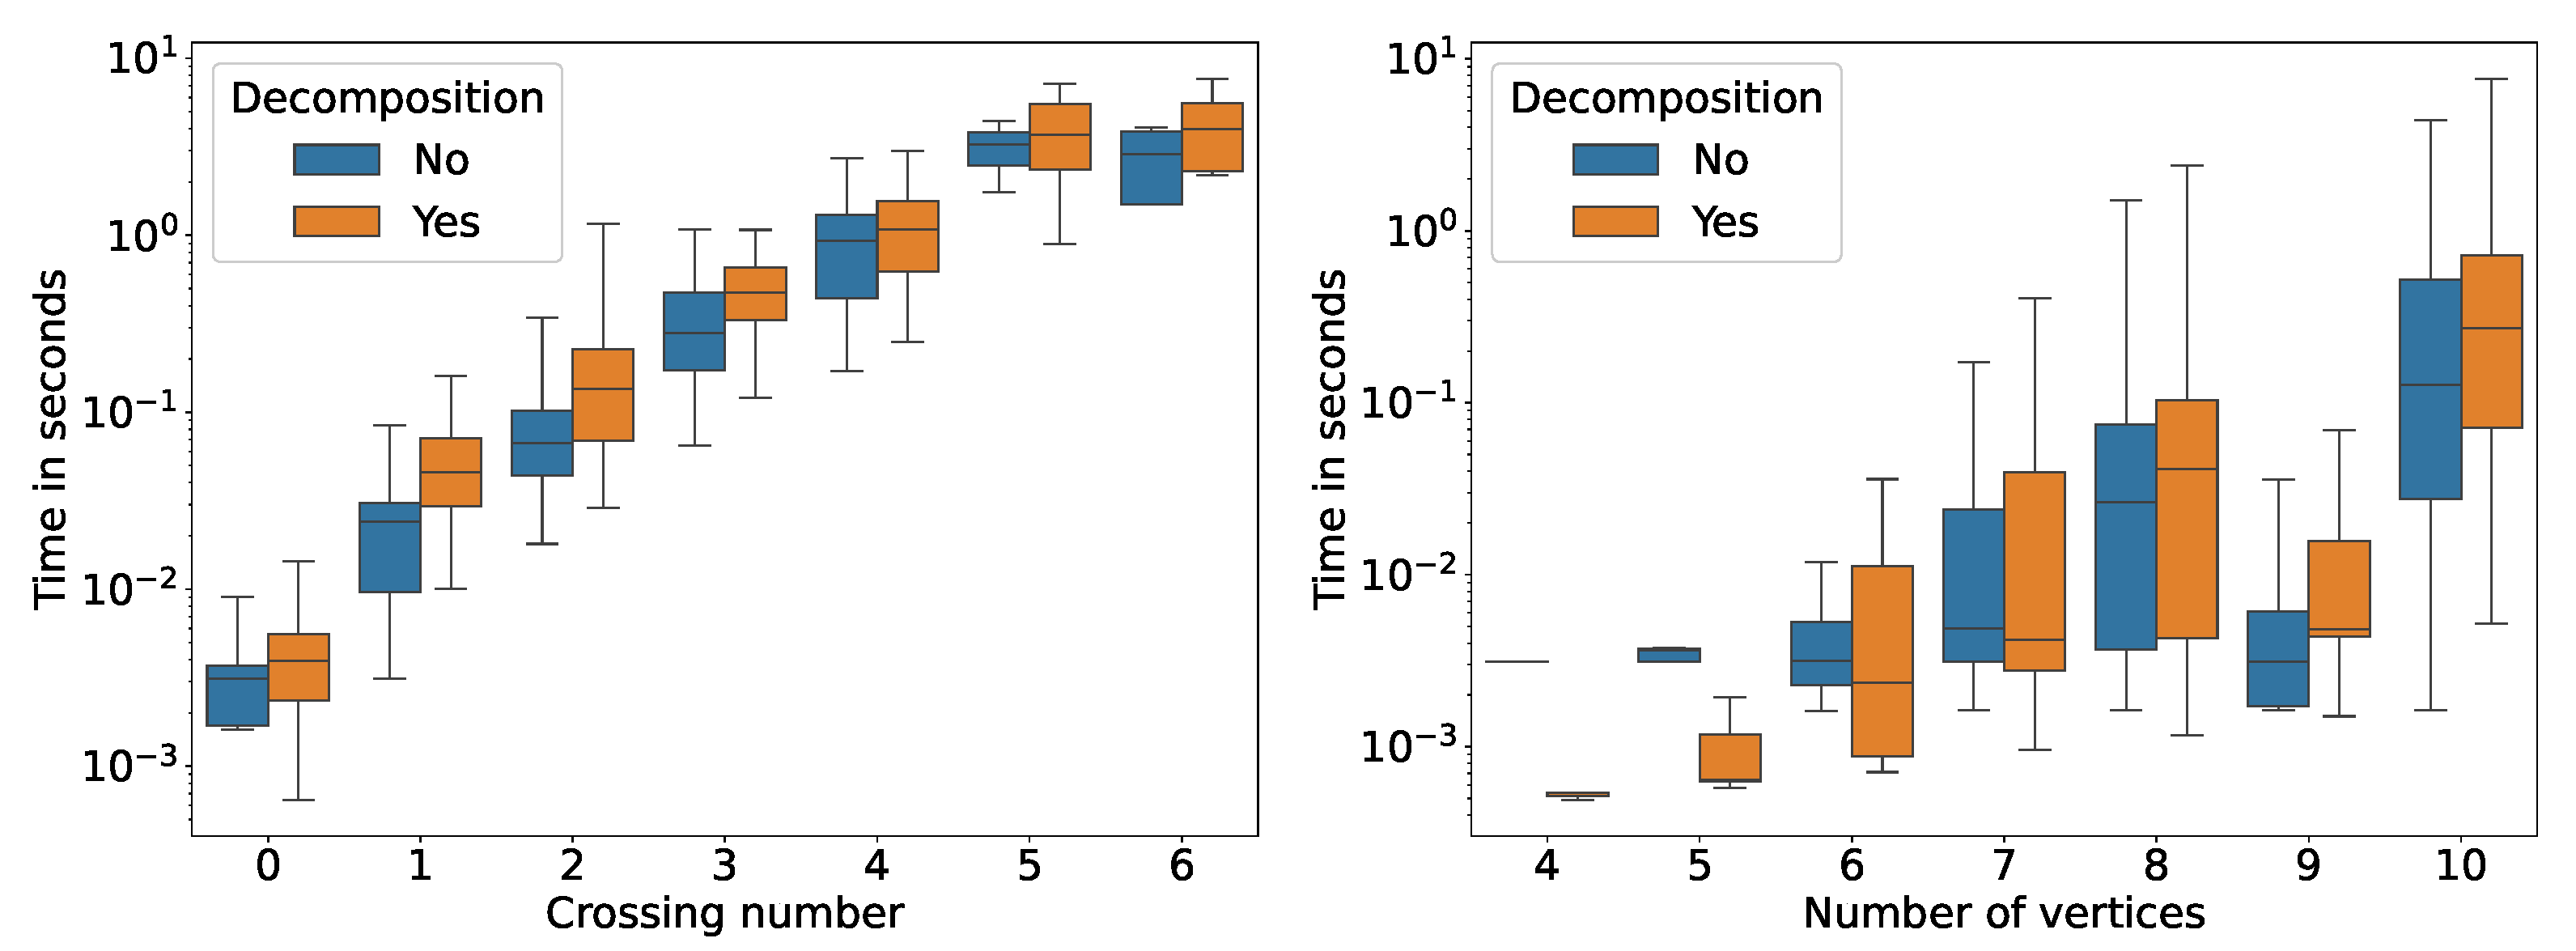
\includegraphics[width=.97\textwidth]{experiments/bctree_ilp}
    } \hfill
    \subfloat[\textsf{SAT}]{
        \label{fig:bctree-results:sat}
        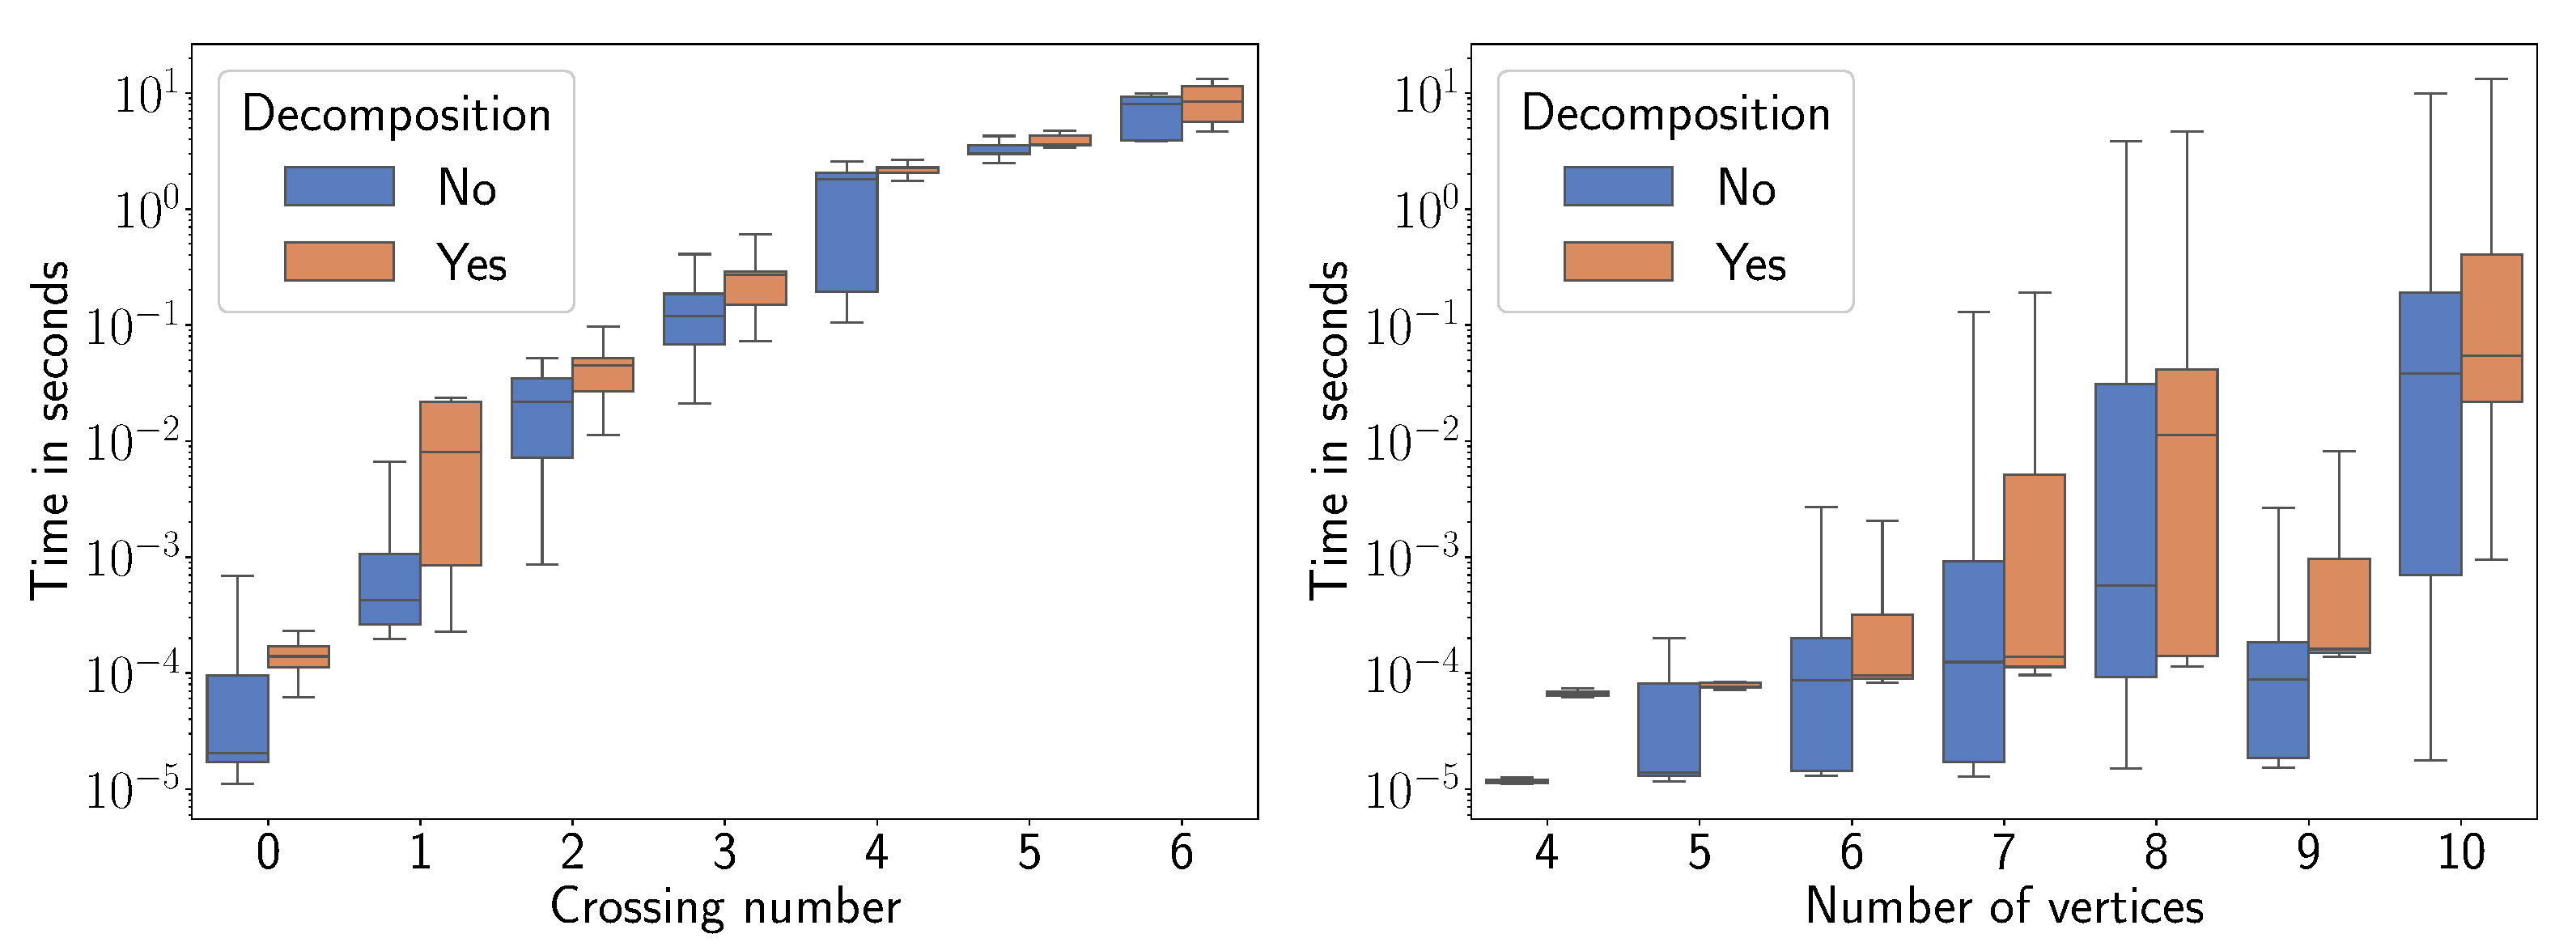
\includegraphics[width=.97\textwidth]{experiments/bctree_sat}
    } \hfill
    \subfloat[\textsf{DP}]{
        \label{fig:bctree-results:okp}
        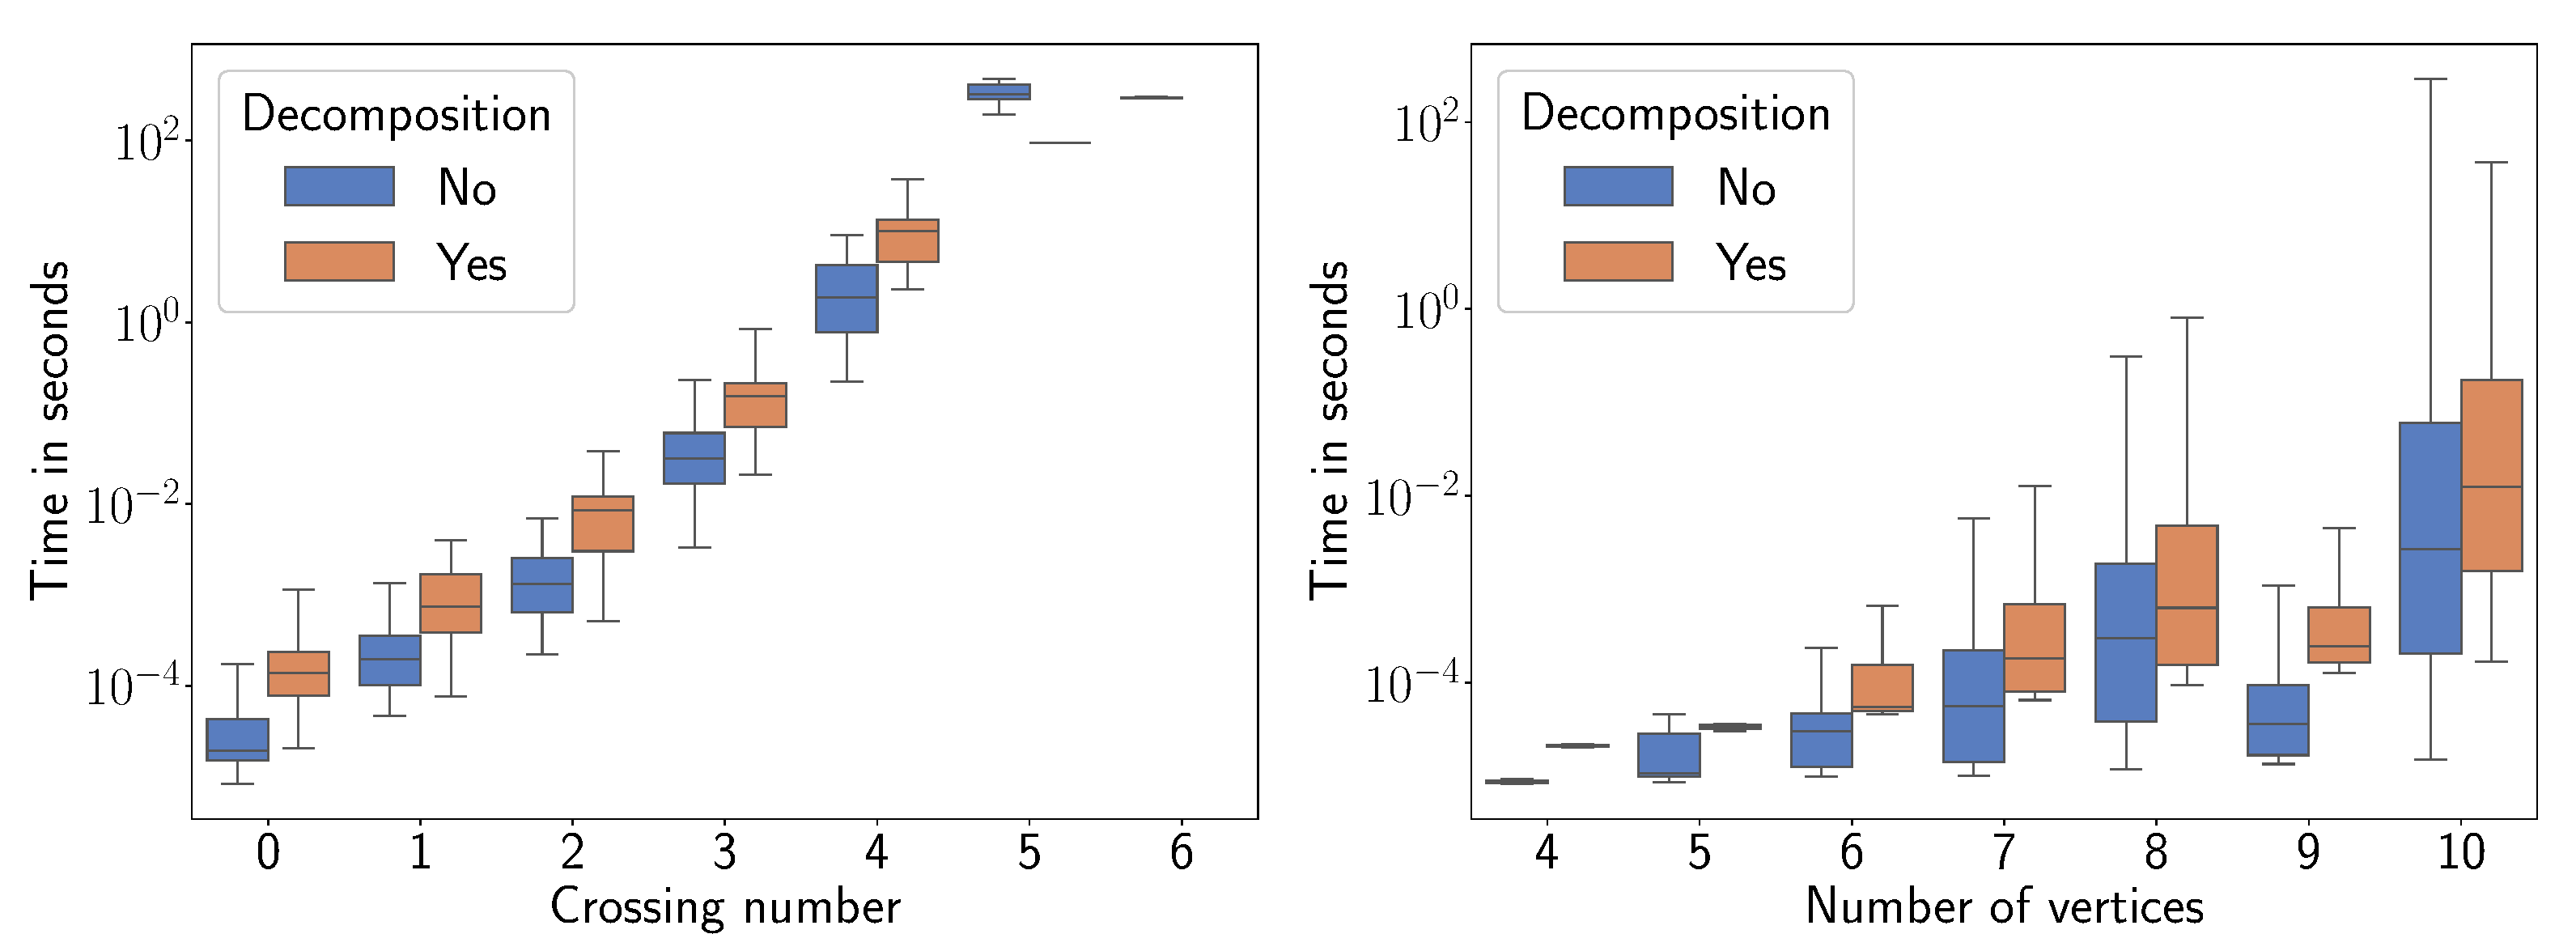
\includegraphics[width=.97\textwidth]{experiments/bctree_okp}
    }
    \caption{Results of the experiment, demonstrating the influence of biconnected decomposition on the running time of \textsf{ILP} , \textsf{SAT} and \textsf{DP}.}
    \label{fig:bctree-results}
\end{figure}

The first experiment we considered was comparing the performance of the algorithms with and without bicomponent decomposition. Here, we used only non-biconnected graphs from the dataset to show the difference between the two configurations. We ran this for all three methods. The results are presented in the~\Cref{fig:bctree-results}.

The results prove that using decomposition indeed boosts performance for almost all methods and graphs. The only exceptions are small graphs for \textsf{ILP}, for which the cost of initialising multiple environments outweighs the cost of decoupling the problem.

As we demonstrated in this experiment, the non-biconnectivity of the graphs artificially decreases the complexity of the recognition task, as each one of them requires multiple times fewer resources compared to equally sized biconnected graphs. Thus, in the following experiments, we consider only biconnected graphs to exclude this source of noise from the results.


\section{Comparison of the algorithms}

In this experiment, we compared the performance of the algorithms. We grouped results by crossing numbers and the algorithm used for solving and displayed in~\Cref{fig:methods}. Due to the complexity of the problem, some runs ran out of allocated resources. So, to display the results, we used only the measurements from runs that successfully found the minimal crossing number. As a result, starting from \(k = 6\), boxes for \textsf{SAT} and \textsf{DP} depict fewer runs compared to \textsf{ILP} as they required more resources for some graphs than were available.

\begin{figure}[tbh]
    \centering
    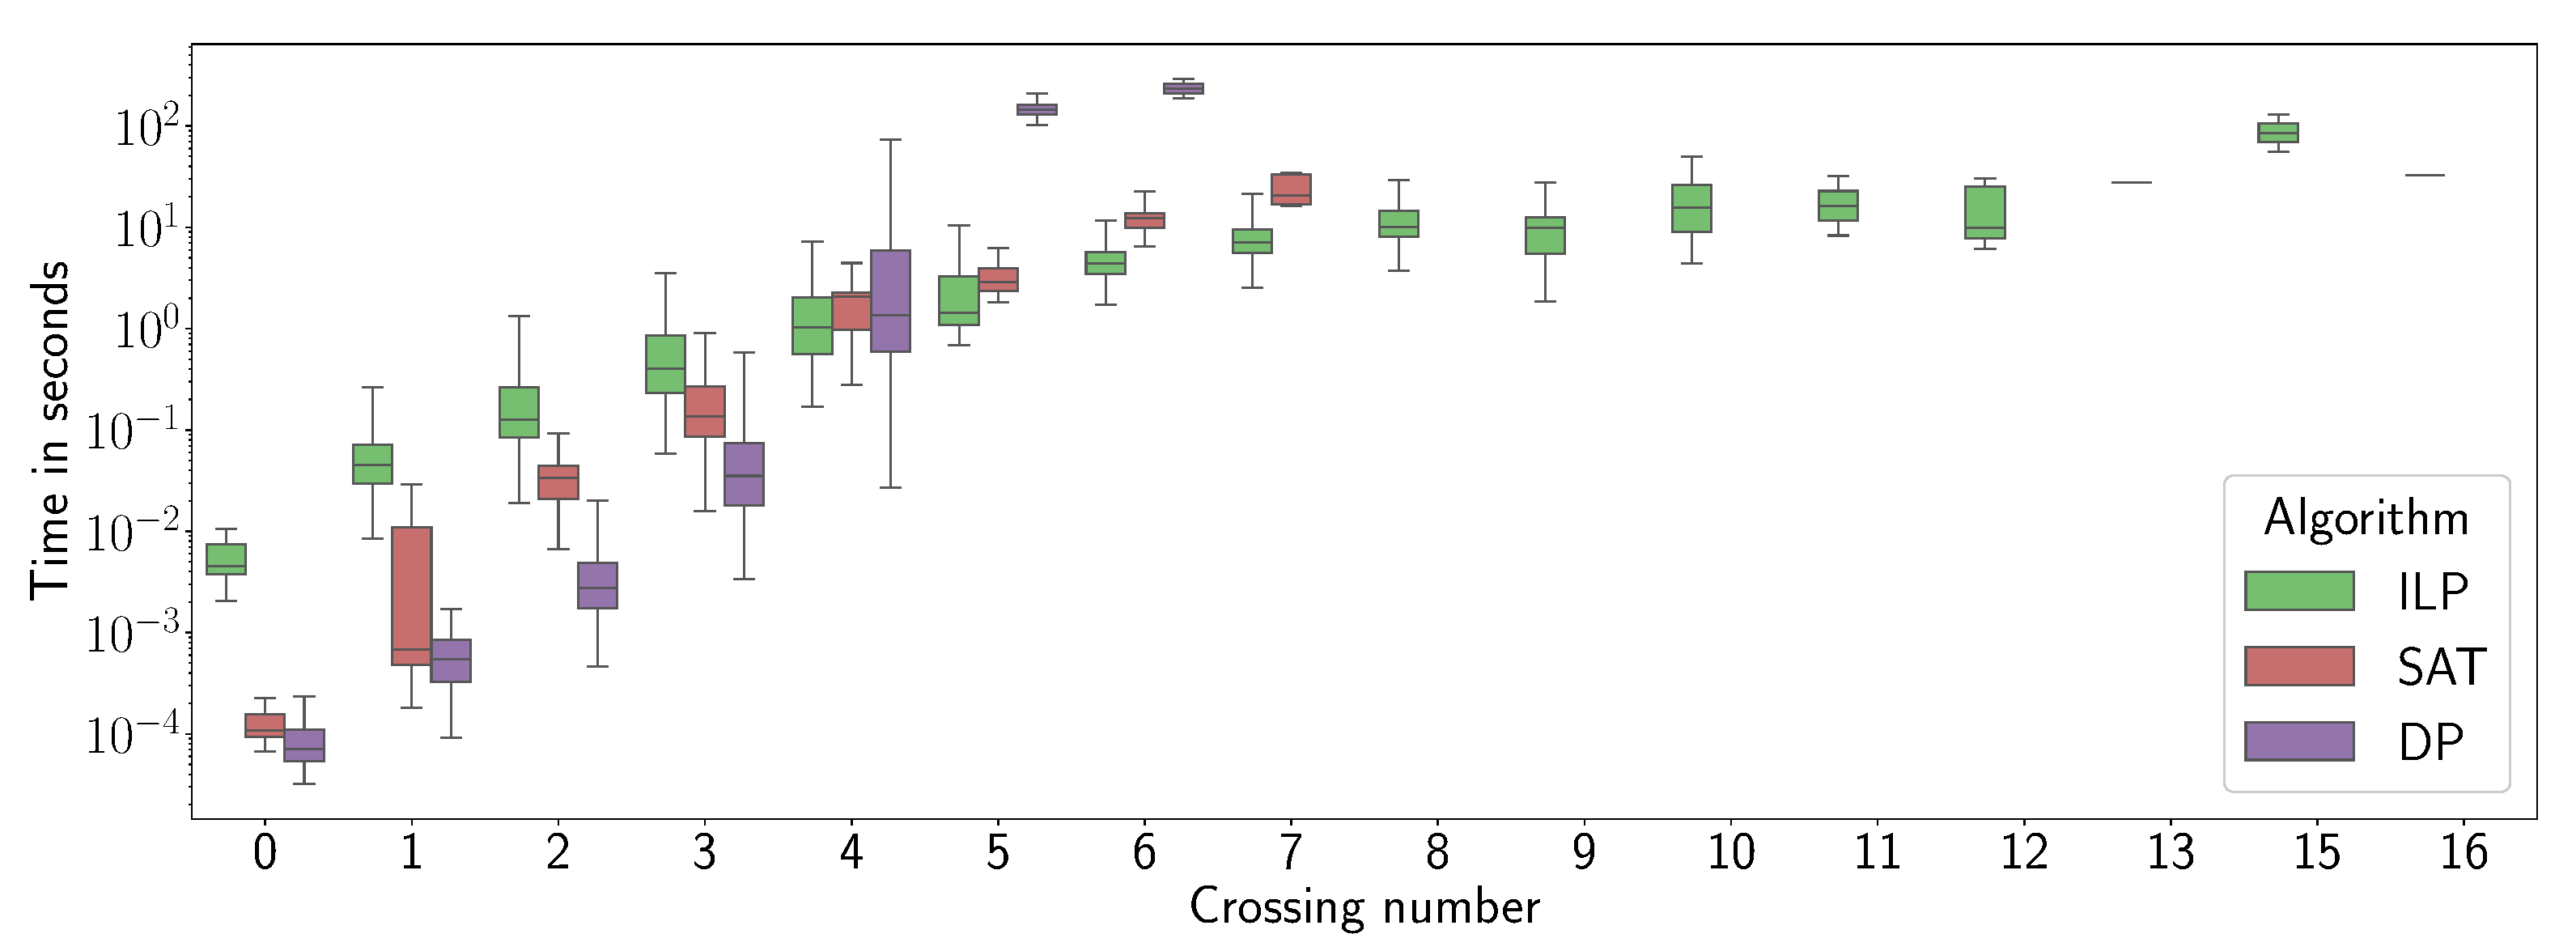
\includegraphics[width=\textwidth]{experiments/methods}
    \caption{Comparison of running times of different algorithms for graphs with different crossing numbers.}
    \label{fig:methods}
\end{figure}

\textsf{SAT} and \textsf{DP}, however, were limited primarily by different factors. Unlike \textsf{ILP}, encoding in \textsf{SAT} contains an exponential number of clauses in terms of circular local crossing number. As a result, the solver ran out of allocated memory for \(185\) out of \(1326\) biconnected graphs. Similarly, \textsf{DP} ran out of memory \(16\) times. However, the bigger limiting factor for this algorithm is time, as \(317\) runs exceeded the 10-minute time limit imposed on each one. All other runs finished successfully.

The results show that the time required by both \textsf{SAT} and \textsf{DP} grows much faster than the time required by \textsf{ILP}. The latter requires each instance to set up an environment for the graphs. With smaller crossing numbers, these costs outweigh the solver's speed. However, for instances with bigger \(k\), the time required for setup is negligible.

\begin{figure}[tbh]
    \centering
    \subfloat[\(k = 2\)]{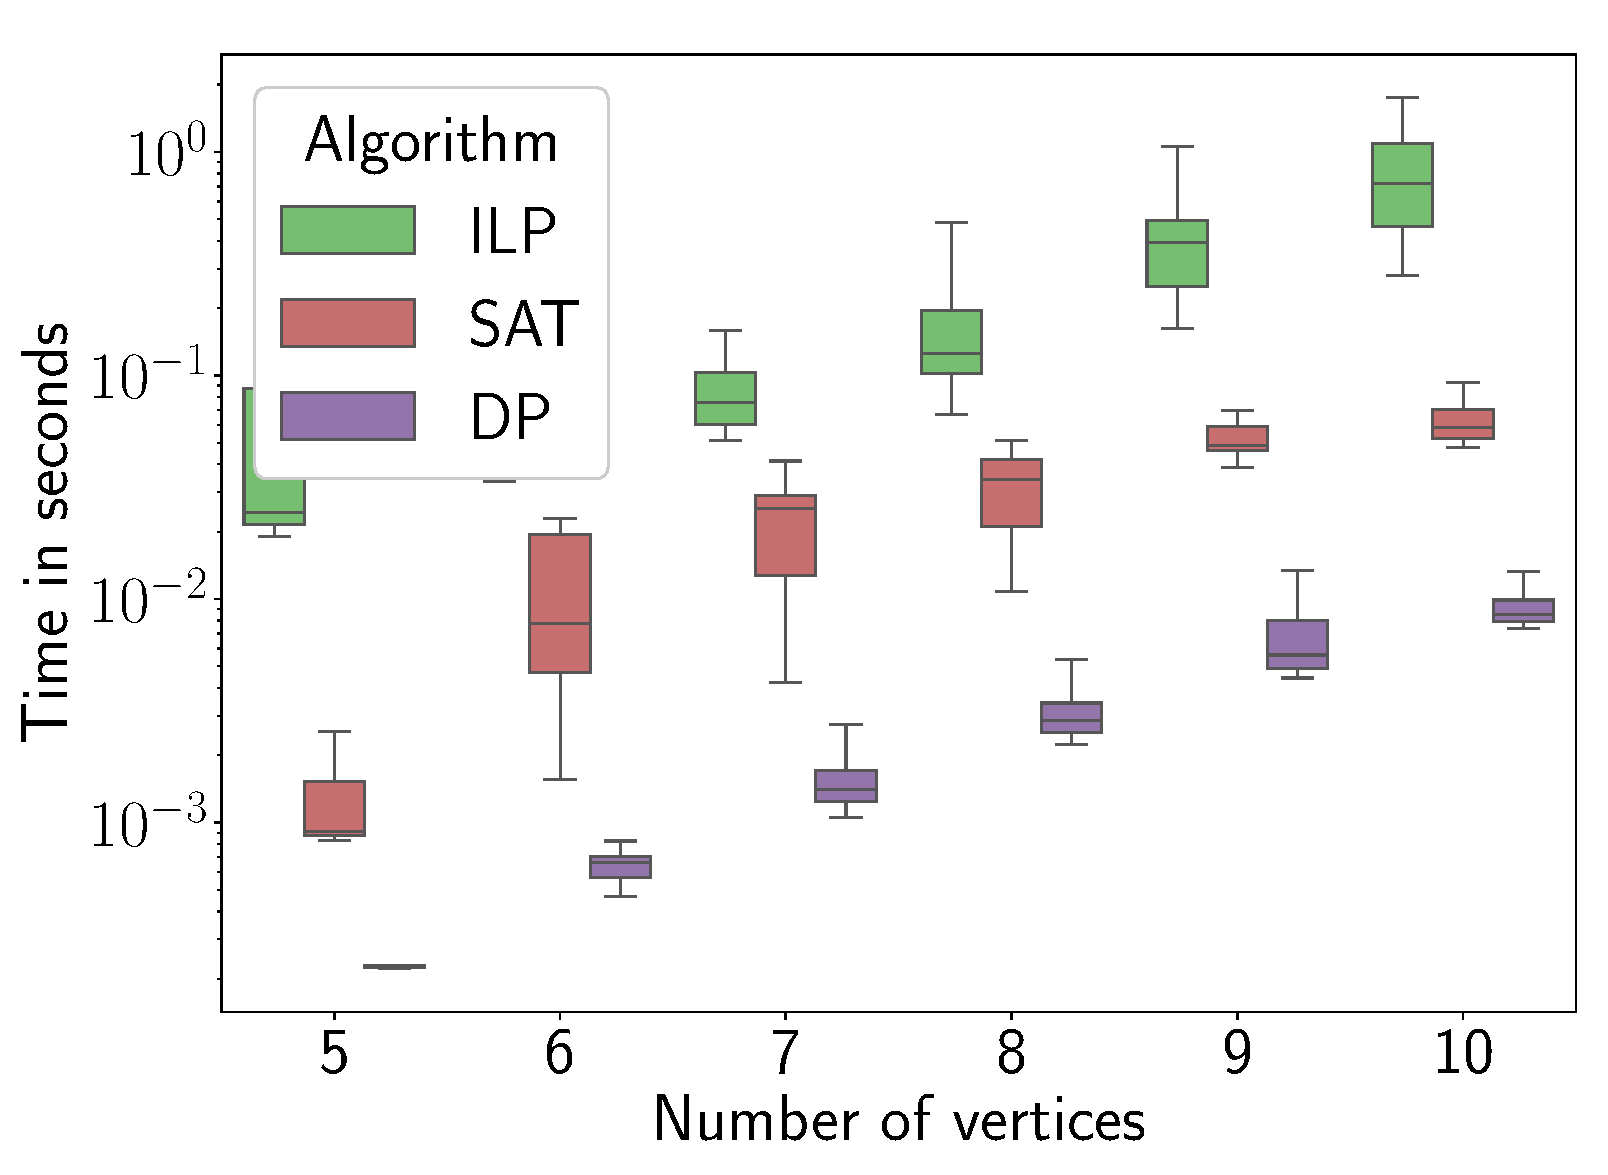
\includegraphics[width=.48\textwidth]{experiments/method_2}} \hfill
    \subfloat[\(k = 3\)]{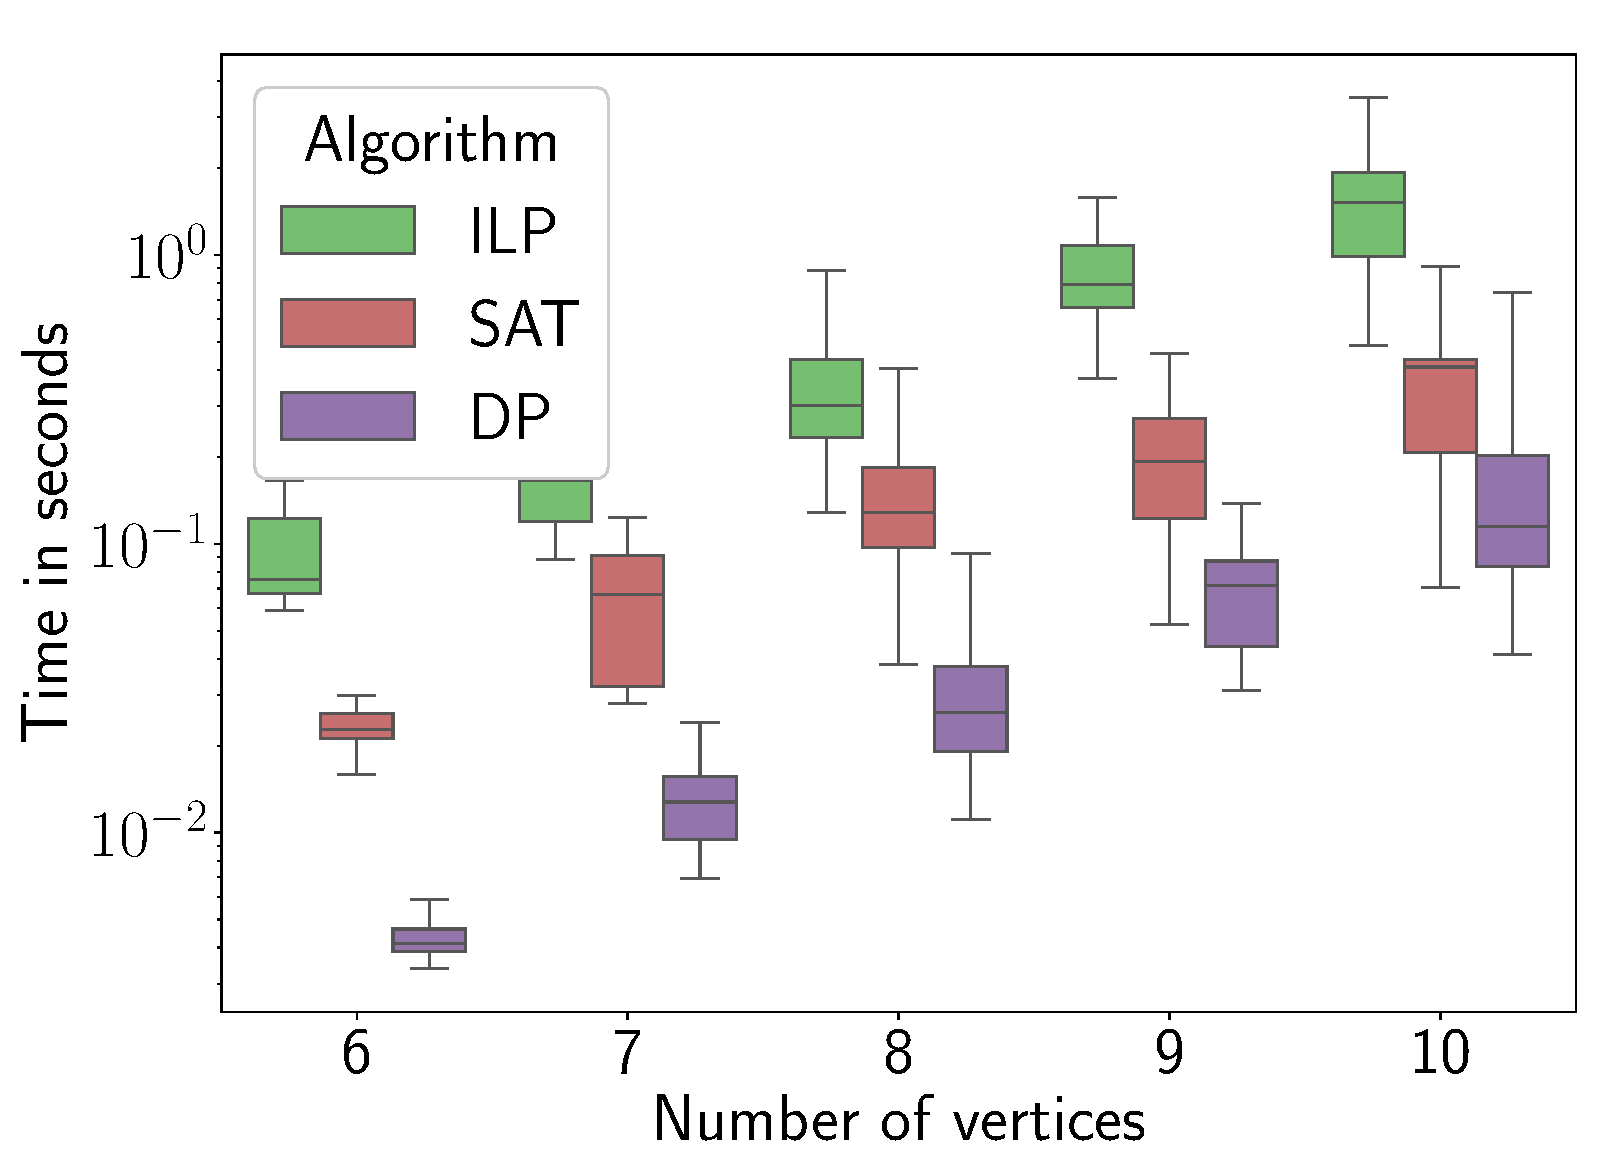
\includegraphics[width=.48\textwidth]{experiments/method_3}} \hfill
    \subfloat[\(k = 4\)]{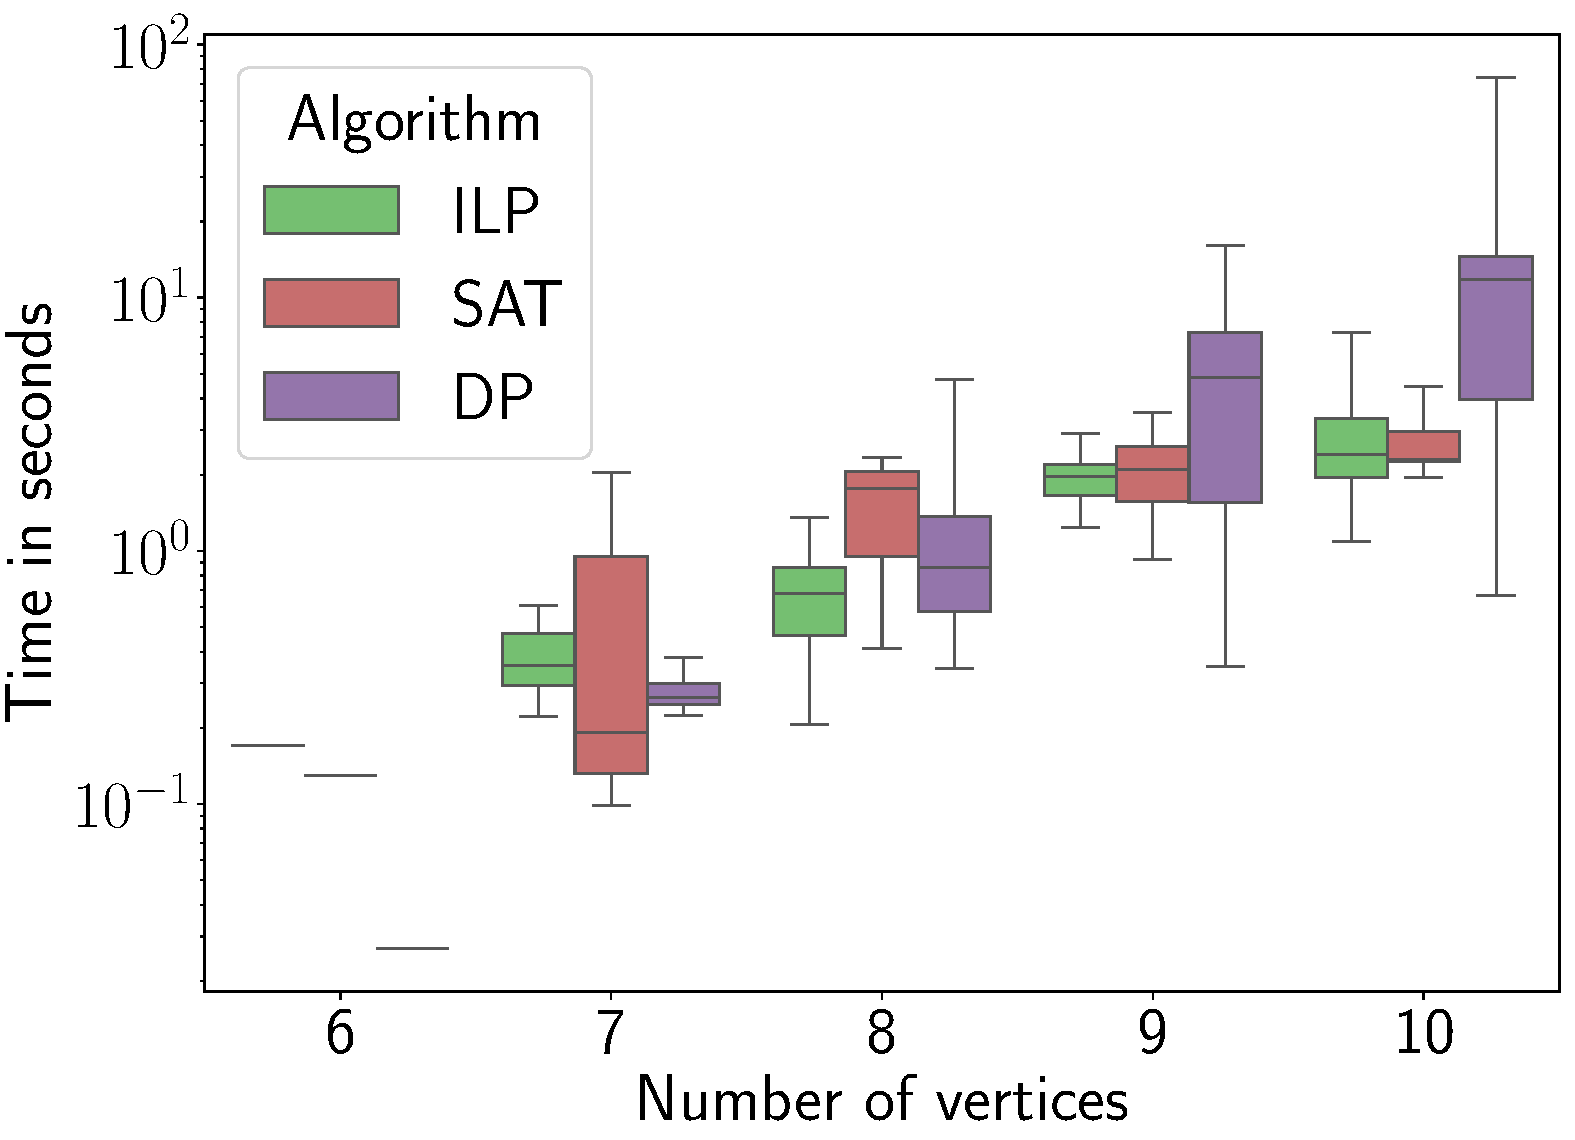
\includegraphics[width=.48\textwidth]{experiments/method_4}} \hfill
    \subfloat[\(k = 5\)]{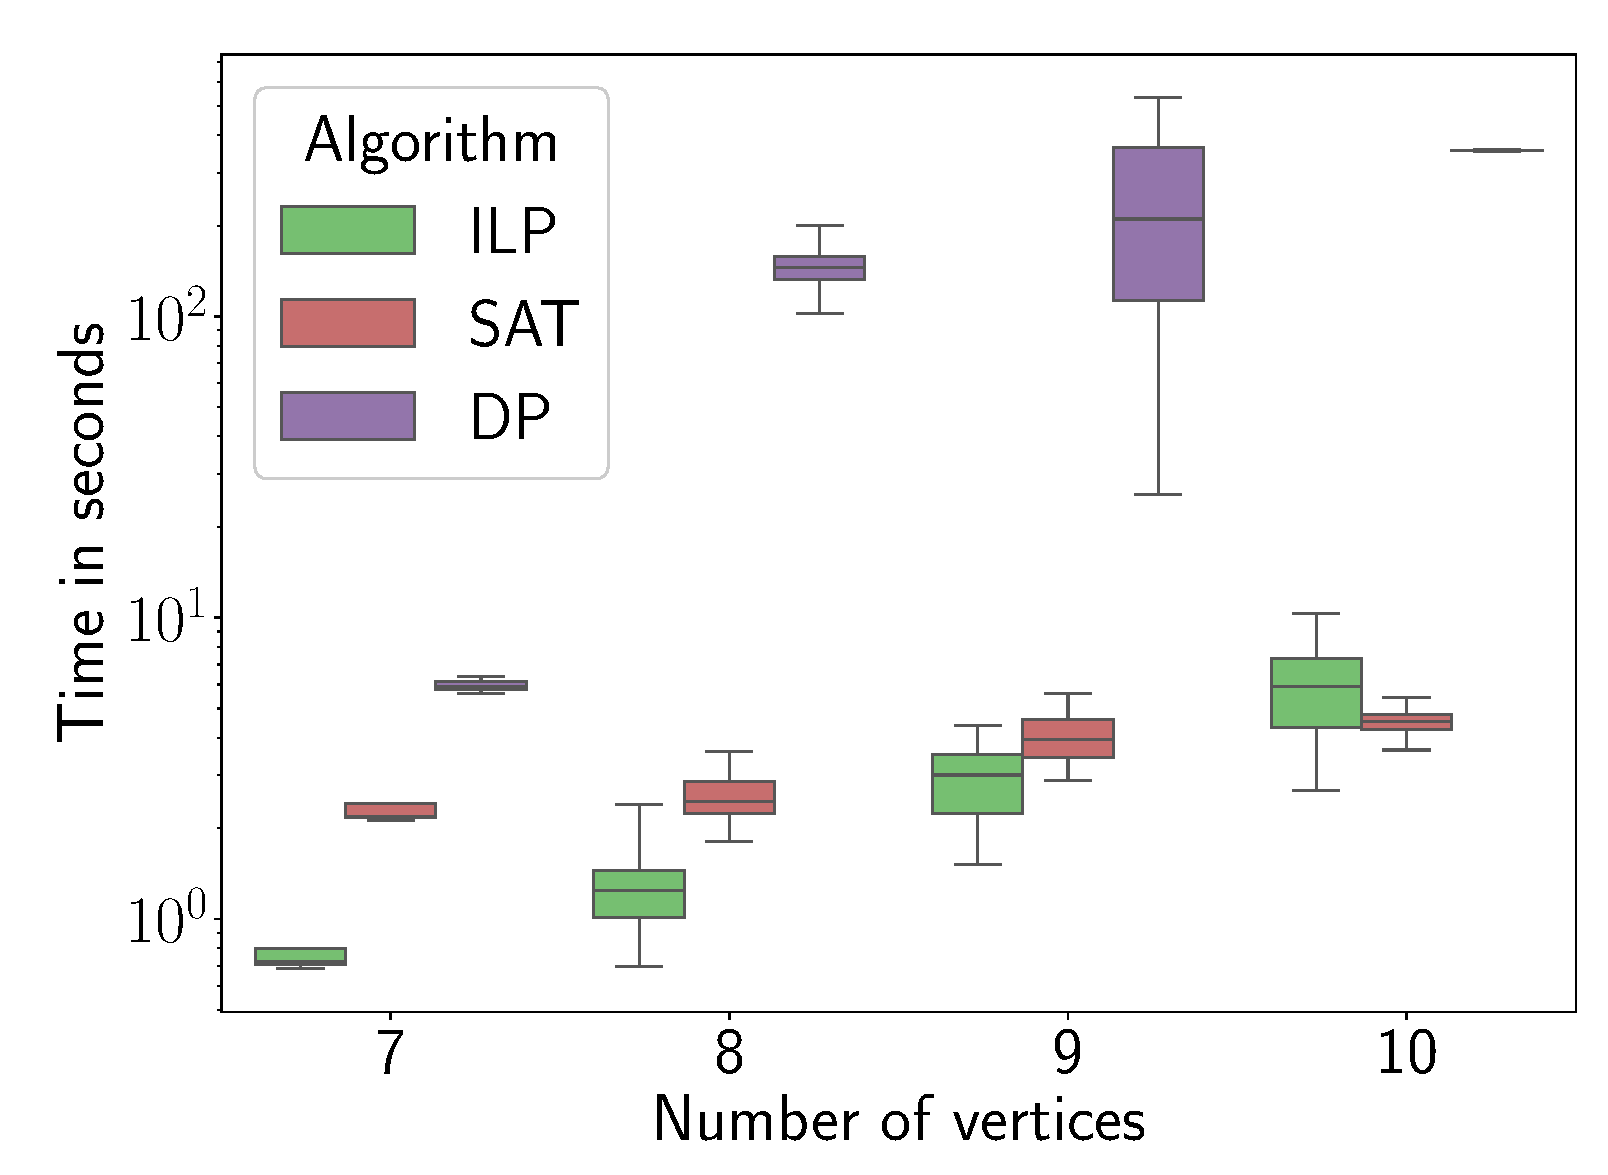
\includegraphics[width=.48\textwidth]{experiments/method_5}} \hfill
    \caption{Comparison of running times required by algorithms to recognise outer \(k\)-planar graphs for various values of \(k\).}
    \label{fig:methods-vertices}
\end{figure}

As the algorithm's running time depends not only on crossing numbers but also on the size of the graph, we can represent the results more accurately by grouping them by both the crossing number and the number of vertices. To demonstrate this dependency, in~\Cref{fig:methods-vertices}, we created a plot for each crossing number represented by at least \(150\) graphs. These plots show that, for \(k \in \{2, 3\}\), \textsf{DP} and \textsf{SAT} are consistently the two fastest methods, with the former being faster than the latter. However, starting from \(k = 4\) and graphs with at least \(9\) vertices, \textsf{ILP} outperforms the other two methods. Most importantly, these results agree with the ones displayed in~\Cref{fig:methods}, which aggregate them for each value \(k\).


\section{Optimisation benchmark}

The last experiment we considered is the comparison of optimisations we discussed for \textsf{ILP} and \textsf{SAT} in~\Cref{sec:optimisations}. For \textsf{ILP}, we ran four configurations for each biconnected graph using none, one, or both optimisations. For \textsf{SAT}, we used two configurations with and without optimisation. The results are presented in~\Cref{fig:optimisation:ilp} and~\Cref{fig:optimisation:sat} respectively.

\begin{figure}[tbh]
    \centering
    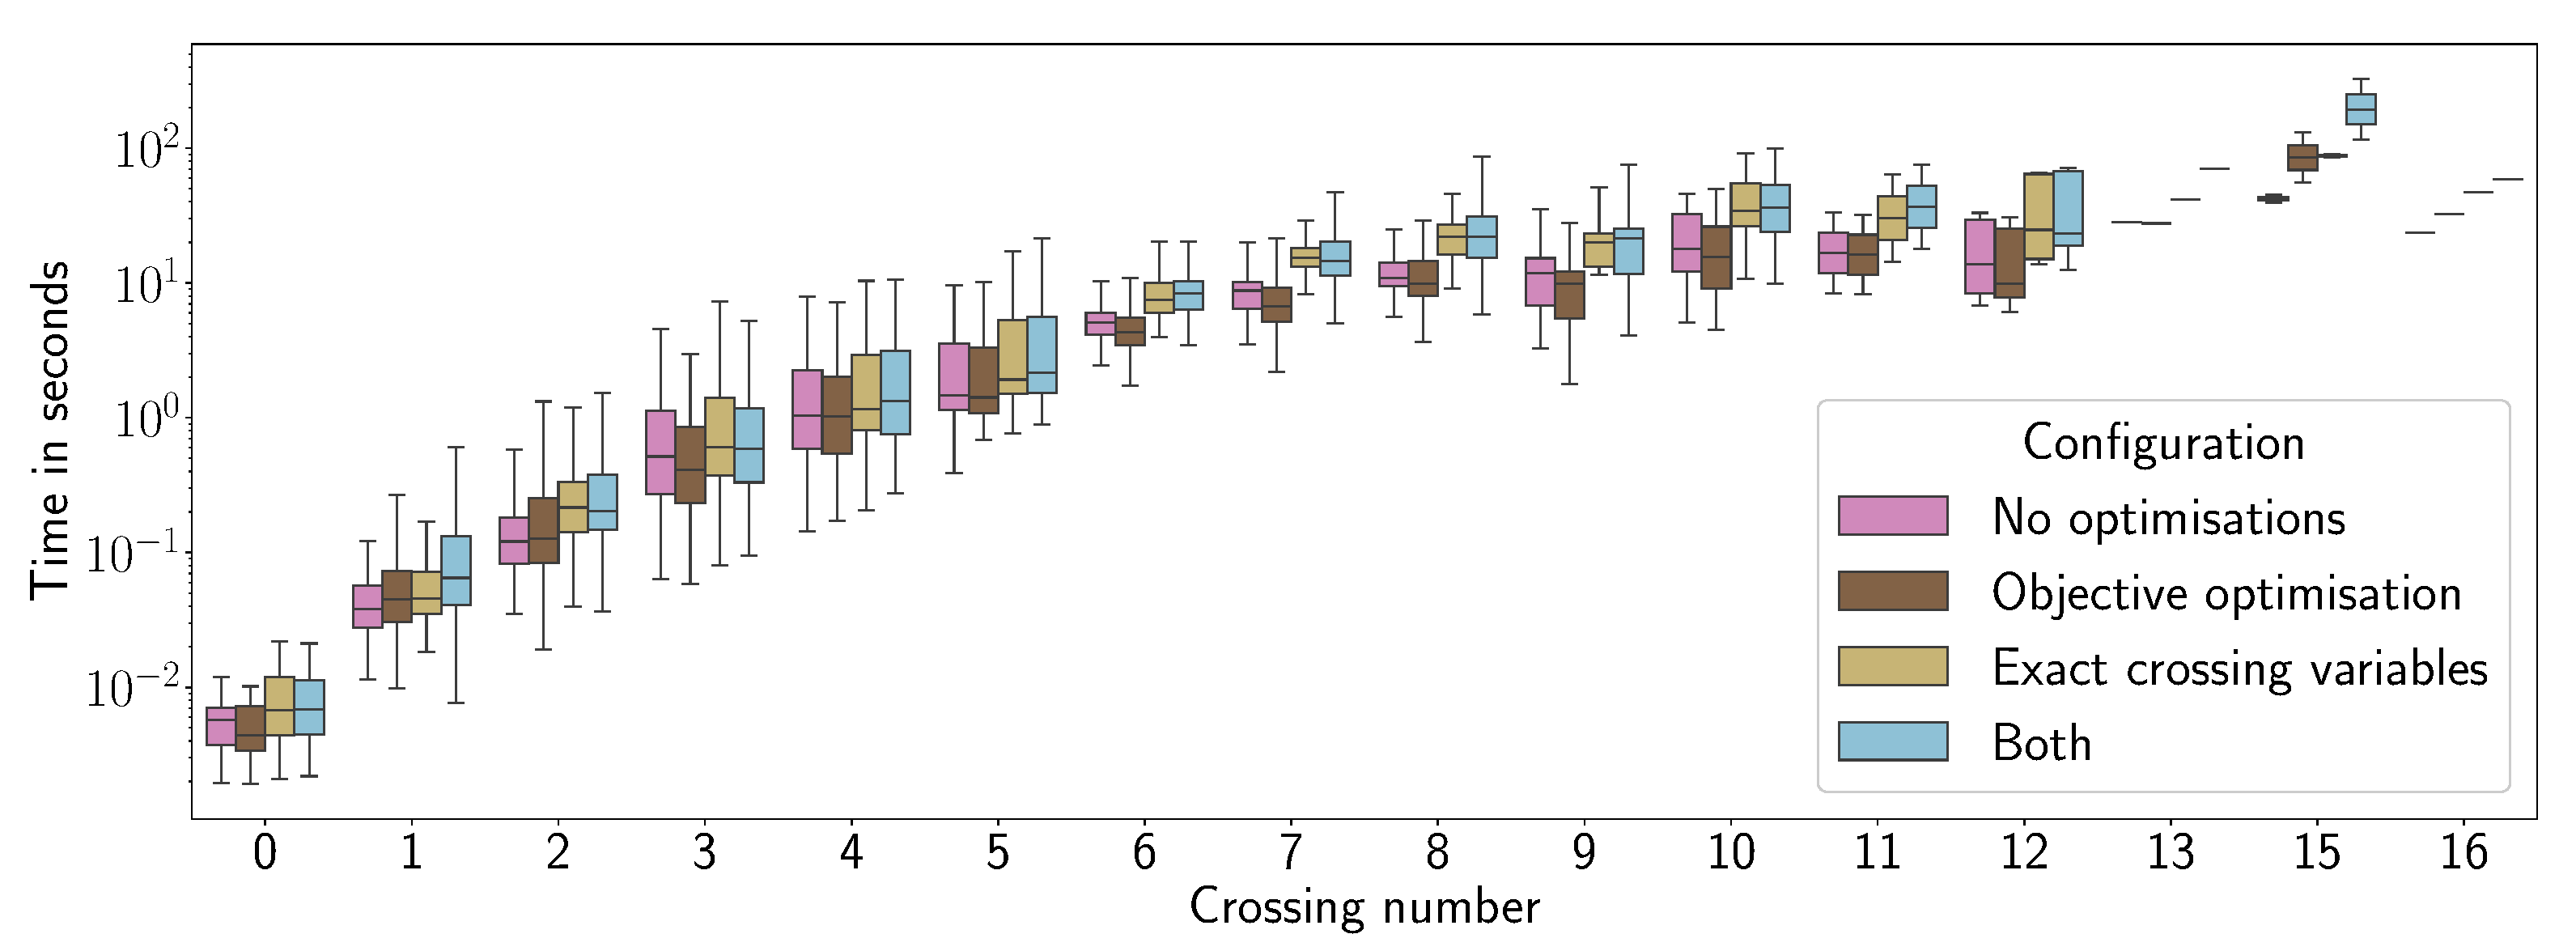
\includegraphics[width=\textwidth]{experiments/ilp}
    \caption{Comparison of different configurations for \textsf{ILP}.}
    \label{fig:optimisation:ilp}
\end{figure}

\begin{figure}[tbh]
    \centering
    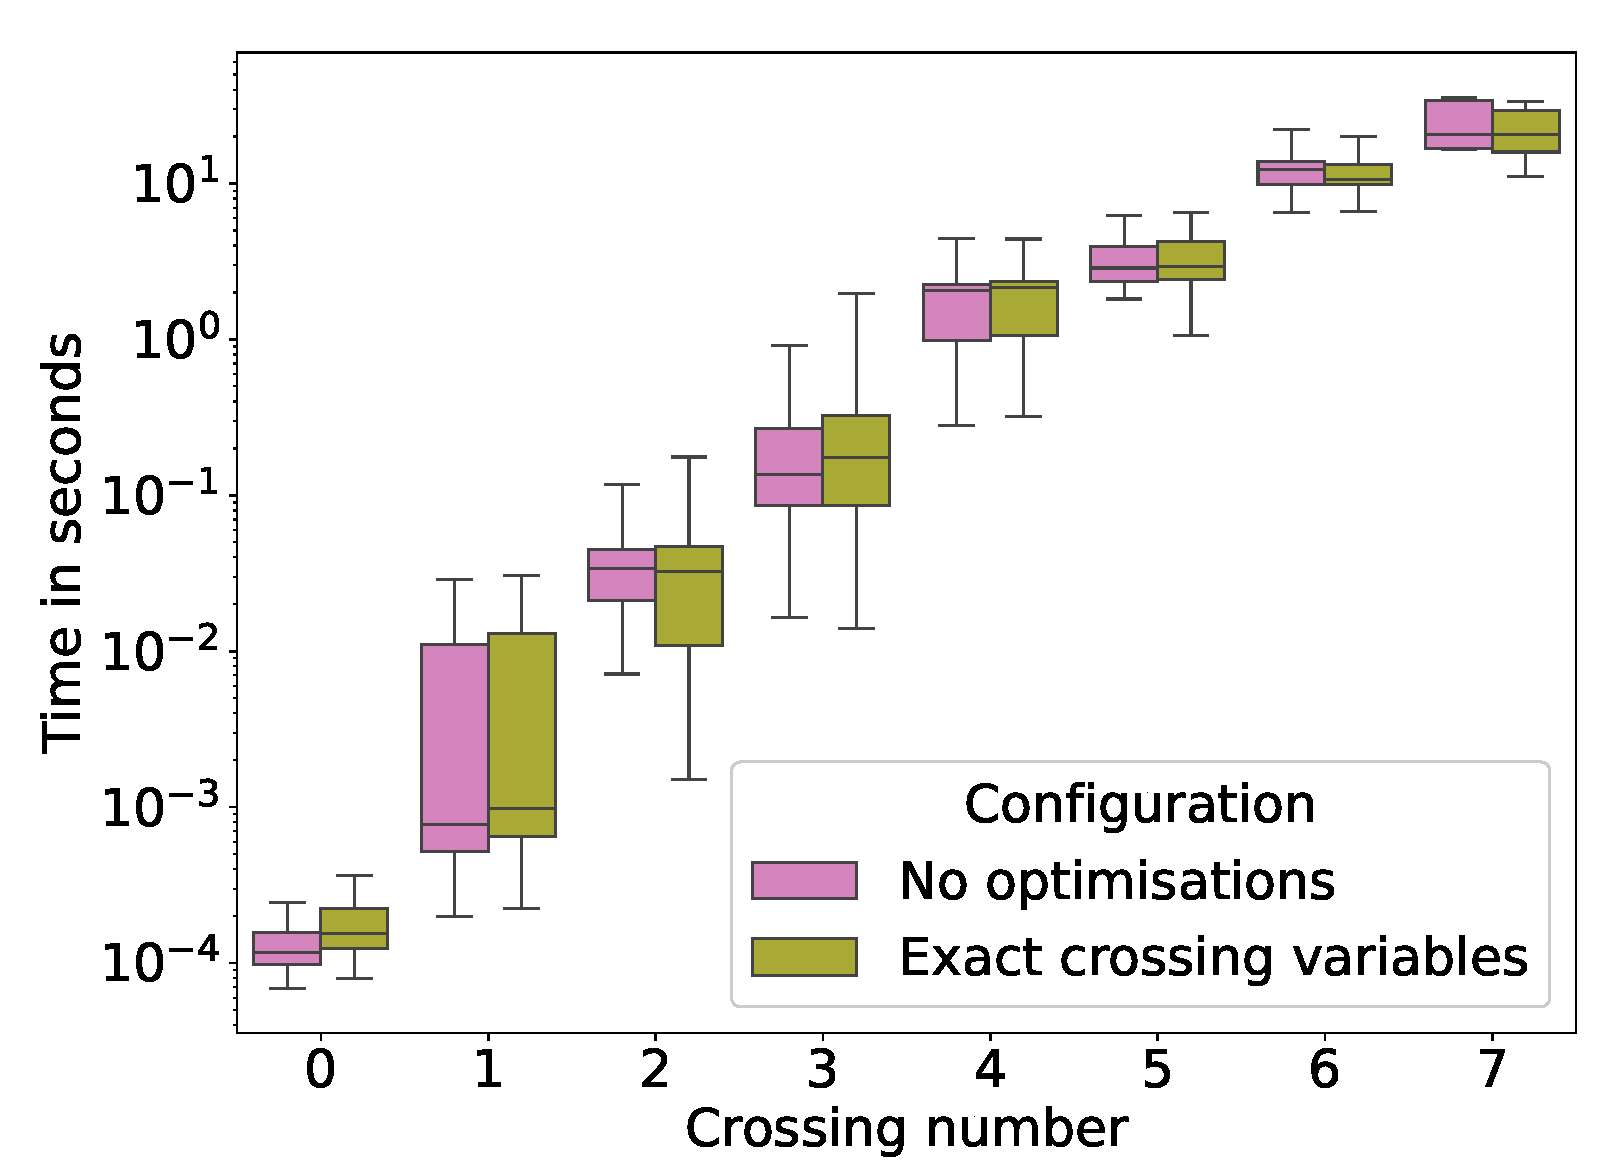
\includegraphics[width=0.47\textwidth]{experiments/sat}
    \caption{Comparison of different configurations for \textsf{SAT}.}
    \label{fig:optimisation:sat}
\end{figure}

In the first plot, we can clearly see that adding additional constraints to enforce the exact value for each crossing variable degrades the performance. For \textsf{SAT}, however, this change does not influence this much. We can see a slight rise in execution time, but the difference is within the margin of error. Here, the difference may be caused by the algorithm writing down the required additional constraints, not the SAT solver.

The objective optimisation for \textsf{ILP}, which includes an extra term in the objective function, makes small but still an improvement. As a result, we consider the algorithm that includes this optimisation to be the most efficient \textsf{ILP}. Thus, we have used this configuration for all other experiments. For \textsf{SAT}, we used a configuration that did not include optimisation.

    \chapter{Conclusions}\label{ch:conclusions}

In this bachelor thesis, we have provided implementations of three algorithms for recognising outer \(k\)-planar graphs. Two of them are based on integer linear programming and satisfiability formulation and have been introduced in this thesis. The last one uses a dynamic programming approach, recently presented by \citeauthor{okp}~\cite{okp}. Additionally, we provide a command line tool to invoke the desired method for a specific graph \(G\). The tool returns the local circular crossing number \(k\) of \(G\) together with a circular drawing of \(G\) where each edge is intersected at most \(k\) times.

We have also demonstrated an example of the program's output for a sample graph and the results of the experiments designed to test, evaluate the performance and compare the algorithms with each other. After having analysed the results of the experiments, we conclude as follows:
\begin{itemize}
    \item Despite the overhead required to perform the biconnected decomposition, doing so significantly improves the performance of all methods.
    \item In the ILP-based algorithm, including constraints for all arrangements of two edges' endpoints significantly worsens its performance. On the other hand, including an extra symetry-breaking term in the objective function slightly improves the performance.
    \item In the SAT-based algorithm, including clauses for all arrangements does not influence the performance.
    \item The computational resources required for executing the ILP-based algorithm grow more slowly compared to both the SAT- and DP-based algorithms with increasing local circular crossing number.
    \item The running times of the SAT- and DP-based algorithm grow
    exponentially in terms of the local circular crossing number of the graph.
\end{itemize}

\section{Limitations}

The first and most major limitation of our implementations is the complexity of the underlying algorithm. The exponential dependency of the running time on local circular crossing number of the input graph significantly limits the number of graphs for which using these implementations is practically reasonable.

The current version also limits the number of vertices to \(64\) in the input graph for the DP-based algorithm, as it uses a bitmask for storing subsets of vertices. We implemented this using an integer as a bitmask to lower the memory consumption; hence, this limit may be different for other systems.

\section{Future work}

There are many directions to explore as future work. First of all, we could combine our implementations into a library. By doing so, the algorithms could more easily be called by other programs.

Secondly, we could optimise the underlying algorithms discussed in this work. In particular, it would be desirable to simplify the algorithm for very small values of \(k\). Can outer \(2\)-planar graphs be recognised in, say, quadratic time?

Another direction of improvement might be developing an algorithm that, for the given embedding of an outer \(k\)-planar graph, draws it using Bézier curves for edges instead of straight lines. Using this approach, we can improve the readability of the drawings.

Finally, we can explore the options for further optimisations of the implemented algorithms. One of the highly promising directions to do so would be to make the implementation of the DP-based algorithm multithreaded. By ensuring that all threads check configurations with the right sides of the same size, we eliminate the requirement of memory synchronisation. This makes this algorithm embarrassingly parallel, as it requires synchronising all threads less than \(|V(G)|\) times throughout the whole execution.


%----------------------------------------------------------------------------------------
%	THESIS CONTENT - APPENDICES
%----------------------------------------------------------------------------------------

    \appendix % Cue to tell LaTeX that the following "chapters" are Appendices

% Include the appendices of the thesis as separate files from the Appendices folder
% Uncomment the lines as you write the Appendices

%\chapter{Appendix}
%\include{Appendices/AppendixB}
%\include{Appendices/AppendixC}

%----------------------------------------------------------------------------------------
%	BIBLIOGRAPHY
%----------------------------------------------------------------------------------------

    \printbibliography[heading=bibintoc]

%----------------------------------------------------------------------------------------

\end{document}  
